\documentclass[journal]{IEEEtran}
\usepackage{cite}
\usepackage{amsmath,amssymb,amsfonts}
\usepackage{graphicx}
\usepackage{textcomp}
\usepackage{xcolor}
\usepackage{booktabs}
\usepackage{placeins}
\usepackage[utf8]{inputenc}
\usepackage[T1]{fontenc}
\usepackage{bm}
\usepackage{mathtools}
\usepackage{amsthm}  % 添加这行到你的包列表中
\usepackage{algorithm}          % 提供 algorithm 浮动体
\usepackage{algorithmic}
\usepackage{hyperref}
\hypersetup{hidelinks}
% \usepackage{algpseudocode}      % 提供算法排版命令
\DeclareMathOperator{\diag}{diag}
\newcommand{\R}{\mathbb{R}}
\newcommand{\C}{\mathbb{C}}
\newcommand{\E}{\mathbb{E}}
\newcommand{\argmin}{\operatorname{arg\,min}}
\newcommand{\norm}[1]{\left\|#1\right\|}

%  定义定理类环境
\newtheorem{theorem}{Theorem}
\newtheorem{corollary}{Corollary}
\newtheorem{definition}{Definition}
\newtheorem{example}{Example}

% 添加这行定义 remark 环境
\newtheorem{remark}{Remark}  

\def\BibTeX{{\rm B\kern-.05em{\sc i\kern-.025em b}\kern-.08em
    T\kern-.1667em\lower.7ex\hbox{E}\kern-.125emX}}


\begin{document}

\title{Reference-Assisted Phase Retrieval for Holographic MIMO Reception: Unique Channel and Finite-Alphabet Symbol Recovery}

% \author{Miyu Feng, Shiwei Guo, Tiebin Mi, and Robert Caiming Qiu%
% \thanks{Miyu Feng, Shiwei Guo, Tiebin Mi, and Robert Caiming Qiu are with the
% School of Electronic Information and Communications, Huazhong University of
% Science and Technology, Wuhan, China (e-mail:
% \{miyu\_feng, m202673223, mitiebin, caiming\}@hust.edu.cn).}%
% }


\maketitle

\begin{abstract}
This paper develops a reference-assisted phase-retrieval framework for
holographic MIMO reception from intensity-only measurements, jointly addressing
continuous channel sensing and finite-alphabet data recovery from intensity-only
measurements. A controllable RF reference is superimposed element-wise with the incident field before
square-law detection, breaking the global-phase invariance without coherent
I/Q acquisition. For the resulting affine intensity model, we establish an
exact secant identity and derive Jacobian-based identifiability and stability
conditions for continuous channel parameters. For finite-alphabet signaling,
we show that noiseless symbol recovery is unique if and only if the minimum
energy-domain distance is positive, and derive corresponding pairwise-error and
stability bounds. A spatial four-phase reference code yields an average
separation guarantee and reveals that severe reference--signal energy imbalance
weakens phase information. Guided by these results, a two-stage receiver combines
linearized intensity-domain initialization, stability-guided adaptive training,
damped Gauss--Newton channel estimation, and distance-certified
Gerchberg--Saxton symbol detection. Simulations verify the theoretical
conditions and show that, at $10$~dB, the adaptive policy uses $20.0$ pilot
symbols on average instead of the fixed budget of $40$ while attaining
$-28.1$~dB channel NMSE; the proposed distance metric also predicts
finite-alphabet detection reliability.
\end{abstract}

\begin{IEEEkeywords}
Holographic MIMO, reference-assisted phase retrieval, channel identifiability, finite-alphabet symbol recovery, intensity-only measurements.
\end{IEEEkeywords}

\section{Introduction}
\label{sec:introduction}

Reconfigurable intelligent surfaces (RISs) provide a programmable electromagnetic interface for controlling wireless propagation with low-complexity surface elements. Their operating principles, communication models, and potential gains in coverage and energy efficiency have been extensively studied \cite{wu2019intelligent,di2019reconfigurable,b13,basar2019wireless,huang2019energy,direnzo2020smart,pan2021ris,bjornson2022ris,direnzo2022communication}. Beyond conventional reflecting architectures, densely sampled large intelligent and holographic surfaces can act as spatially continuous apertures, offering high spatial resolution and new wave-domain processing capabilities \cite{hu2018data,dardari2020large,huang2020holographic,zhang2021holographic}. Recent studies have further explored holography-inspired surface control, wave-domain DOA estimation, and metasurface-enabled sensing and localization \cite{r2,fuhai,NEholo,li2026intelligent,cao2026hybrid}; wavenumber-domain processing provides a complementary framework for modeling and processing quasi-continuous holographic apertures \cite{zhang2026wavenumber}.

A central implementation challenge is that acquiring the complex field at every surface element conventionally requires coherent radio-frequency chains, local-oscillator distribution, and in-phase/quadrature sampling. Power-detector-based architectures instead retain only intensity measurements and can substantially simplify the receiving hardware \cite{shen2020intelligent,huangjd2024CS}. Square-law or direct detection is well established in optical and infrared communication systems \cite{kahn1997wireless,armstrong2009ofdm}; when used for complex-valued radio signals, however, it discards the phase that carries essential channel and symbol information. The resulting inverse problem is therefore a form of phase retrieval.

Phase retrieval has a long history in optics and signal processing \cite{fienup1982phase,shechtman2015phase}. Convex lifting and semidefinite relaxations provide recovery guarantees at the cost of high-dimensional optimization \cite{candes2013phaselift,candes2015phase,waldspurger2015phasecut}, whereas alternating-minimization and gradient-based methods offer more scalable nonconvex alternatives \cite{netrapalli2015alternating,candes2015wirtinger}. Recent deep-unfolding approaches further combine interpretable iterative structure with learned signal priors \cite{liu2026unfolding}. In parallel, fundamental results have characterized the number and structure of measurements required for uniqueness and stable recovery \cite{balan2006signal,bandeira2014saving,eldar2014stability,conca2015algebraic,grohs2020phase}. These results clarify the generic phaseless inverse problem, but its unavoidable global-phase ambiguity remains incompatible with the direct recovery of absolute communication symbols.

A known reference wave can remove this ambiguity by interfering with the unknown field before square-law detection. This principle originates from holography, where the object and reference waves form an intensity pattern that encodes their relative phase \cite{gabor1948new,leith1962wavefronts}; controlled reference phases can provide additional complex-field information \cite{yamaguchi1997phase}. Algebraically, the reference converts homogeneous magnitude measurements into affine magnitude measurements, connecting the receiver considered here to affine phase retrieval \cite{affine_phase_retrieval}. Unlike a conventional coherent local oscillator used after antenna combining, the reference in this architecture participates directly in the element-wise interference pattern.

Phaseless recovery has also been investigated in communication problems such as OFDM channel estimation \cite{ofdm_phase_retrieval}. 
For holographic interference surfaces, prior work has exploited the spatial sum-of-exponentials structure to enable phase-shifting interference suppression and Prony-based multi-user channel segmentation \cite{huangjd2024CS}. 
A subsequent wideband extension further introduced holographic channel inversion together with maximum-likelihood and low-complexity sensing algorithms \cite{huang2026wideband}. 
As is typical for Prony-type estimators, the robustness of such methods under a finite aperture is closely related to the conditioning of the associated pole-recovery and Vandermonde systems, particularly when the spatial frequencies of different users are closely spaced. 
Meanwhile, RIS channel acquisition and codebook design have been extensively studied under conventional complex-baseband observation models \cite{Zhou2024,r1,r3}. 
These studies provide effective channel-sensing and training mechanisms, but they do not characterize the finite-measurement injectivity and stability of the complete affine-intensity mapping, nor do they address the identifiability of finite-alphabet symbols. 
In particular, generic recovery guarantees for continuous-valued signals do not directly reveal when two distinct constellation vectors may produce identical or nearly indistinguishable energy patterns under the joint effects of the reference wave, waveform sampling, and the holographic array manifold.

This paper addresses that gap through a unified reference-assisted phase-retrieval framework for RF holographic reception. We first separate field-domain injectivity from reference-induced intensity separation and derive conditions under which finite-alphabet symbols are uniquely represented by the observed energies. We then introduce an energy-domain minimum-distance metric that quantifies noise robustness and exposes the joint roles of reference coding and spatial sampling. Finally, we develop practical channel-estimation and symbol-detection algorithms whose performance can be interpreted through these identifiability and separation properties.

The main contributions of this paper are summarized as follows:
\begin{itemize}
\item We establish a reference-assisted RF holographic receiver model, in which complex-valued communication symbols are recovered from intensity-only measurements through interference between the unknown field and a spatially coded reference wave.
\item We derive discrete identifiability conditions for reference-assisted phase retrieval over finite constellations and reveal the joint impact of the reference wave, the pulse-shaping matrix, and the receiving-surface array manifold on symbol uniqueness.
\item We introduce an energy-domain minimum distance metric to characterize the stability of symbol recovery and to guide reference-wave and spatial-measurement design.
\item We develop and compare maximum-likelihood and low-complexity phase-retrieval detectors, demonstrating that proper spatial reference coding improves symbol distinguishability and detection performance.
\end{itemize}


\section{System Model}
\label{sec:system_model}

We consider an RF holographic receiver in which $L$ single-antenna users transmit complex baseband symbols to a surface composed of multiple receiving units. Each unit senses the intensity of the interference pattern formed by the incident field and a known reference derived from a common local oscillator \cite{huangjd2024CS,yin2025hisprototype}. Unlike a conventional passive RIS, the surface is an active receiving front end: the reference is routed to the detector inputs rather than used to configure electromagnetic reflection. The receiver first estimates the complex channel parameters and directions of arrival (DOAs) and then uses the resulting channel estimate to recover the transmitted symbols.

The scheduled users are assumed to share a common symbol period and to be
frame- and symbol-time aligned at the receiver using conventional uplink
synchronization procedures, including pilot- or preamble-aided timing
acquisition followed by network-controlled ranging or timing adjustment
\cite{morelli2004timing,sanguinetti2009robust}. After synchronization, residual
user-dependent timing offsets are assumed small enough that their effects on
the subslot-integrated measurements can be neglected. Residual
carrier-frequency offsets are likewise assumed sufficiently small for the
received complex fields to remain approximately invariant over one detection
interval. Users that do not satisfy these timing
conditions, such as asynchronous random-access users with unknown relative
delays, are outside the scope of the present model.

\begin{figure}[htbp]
    \centering
    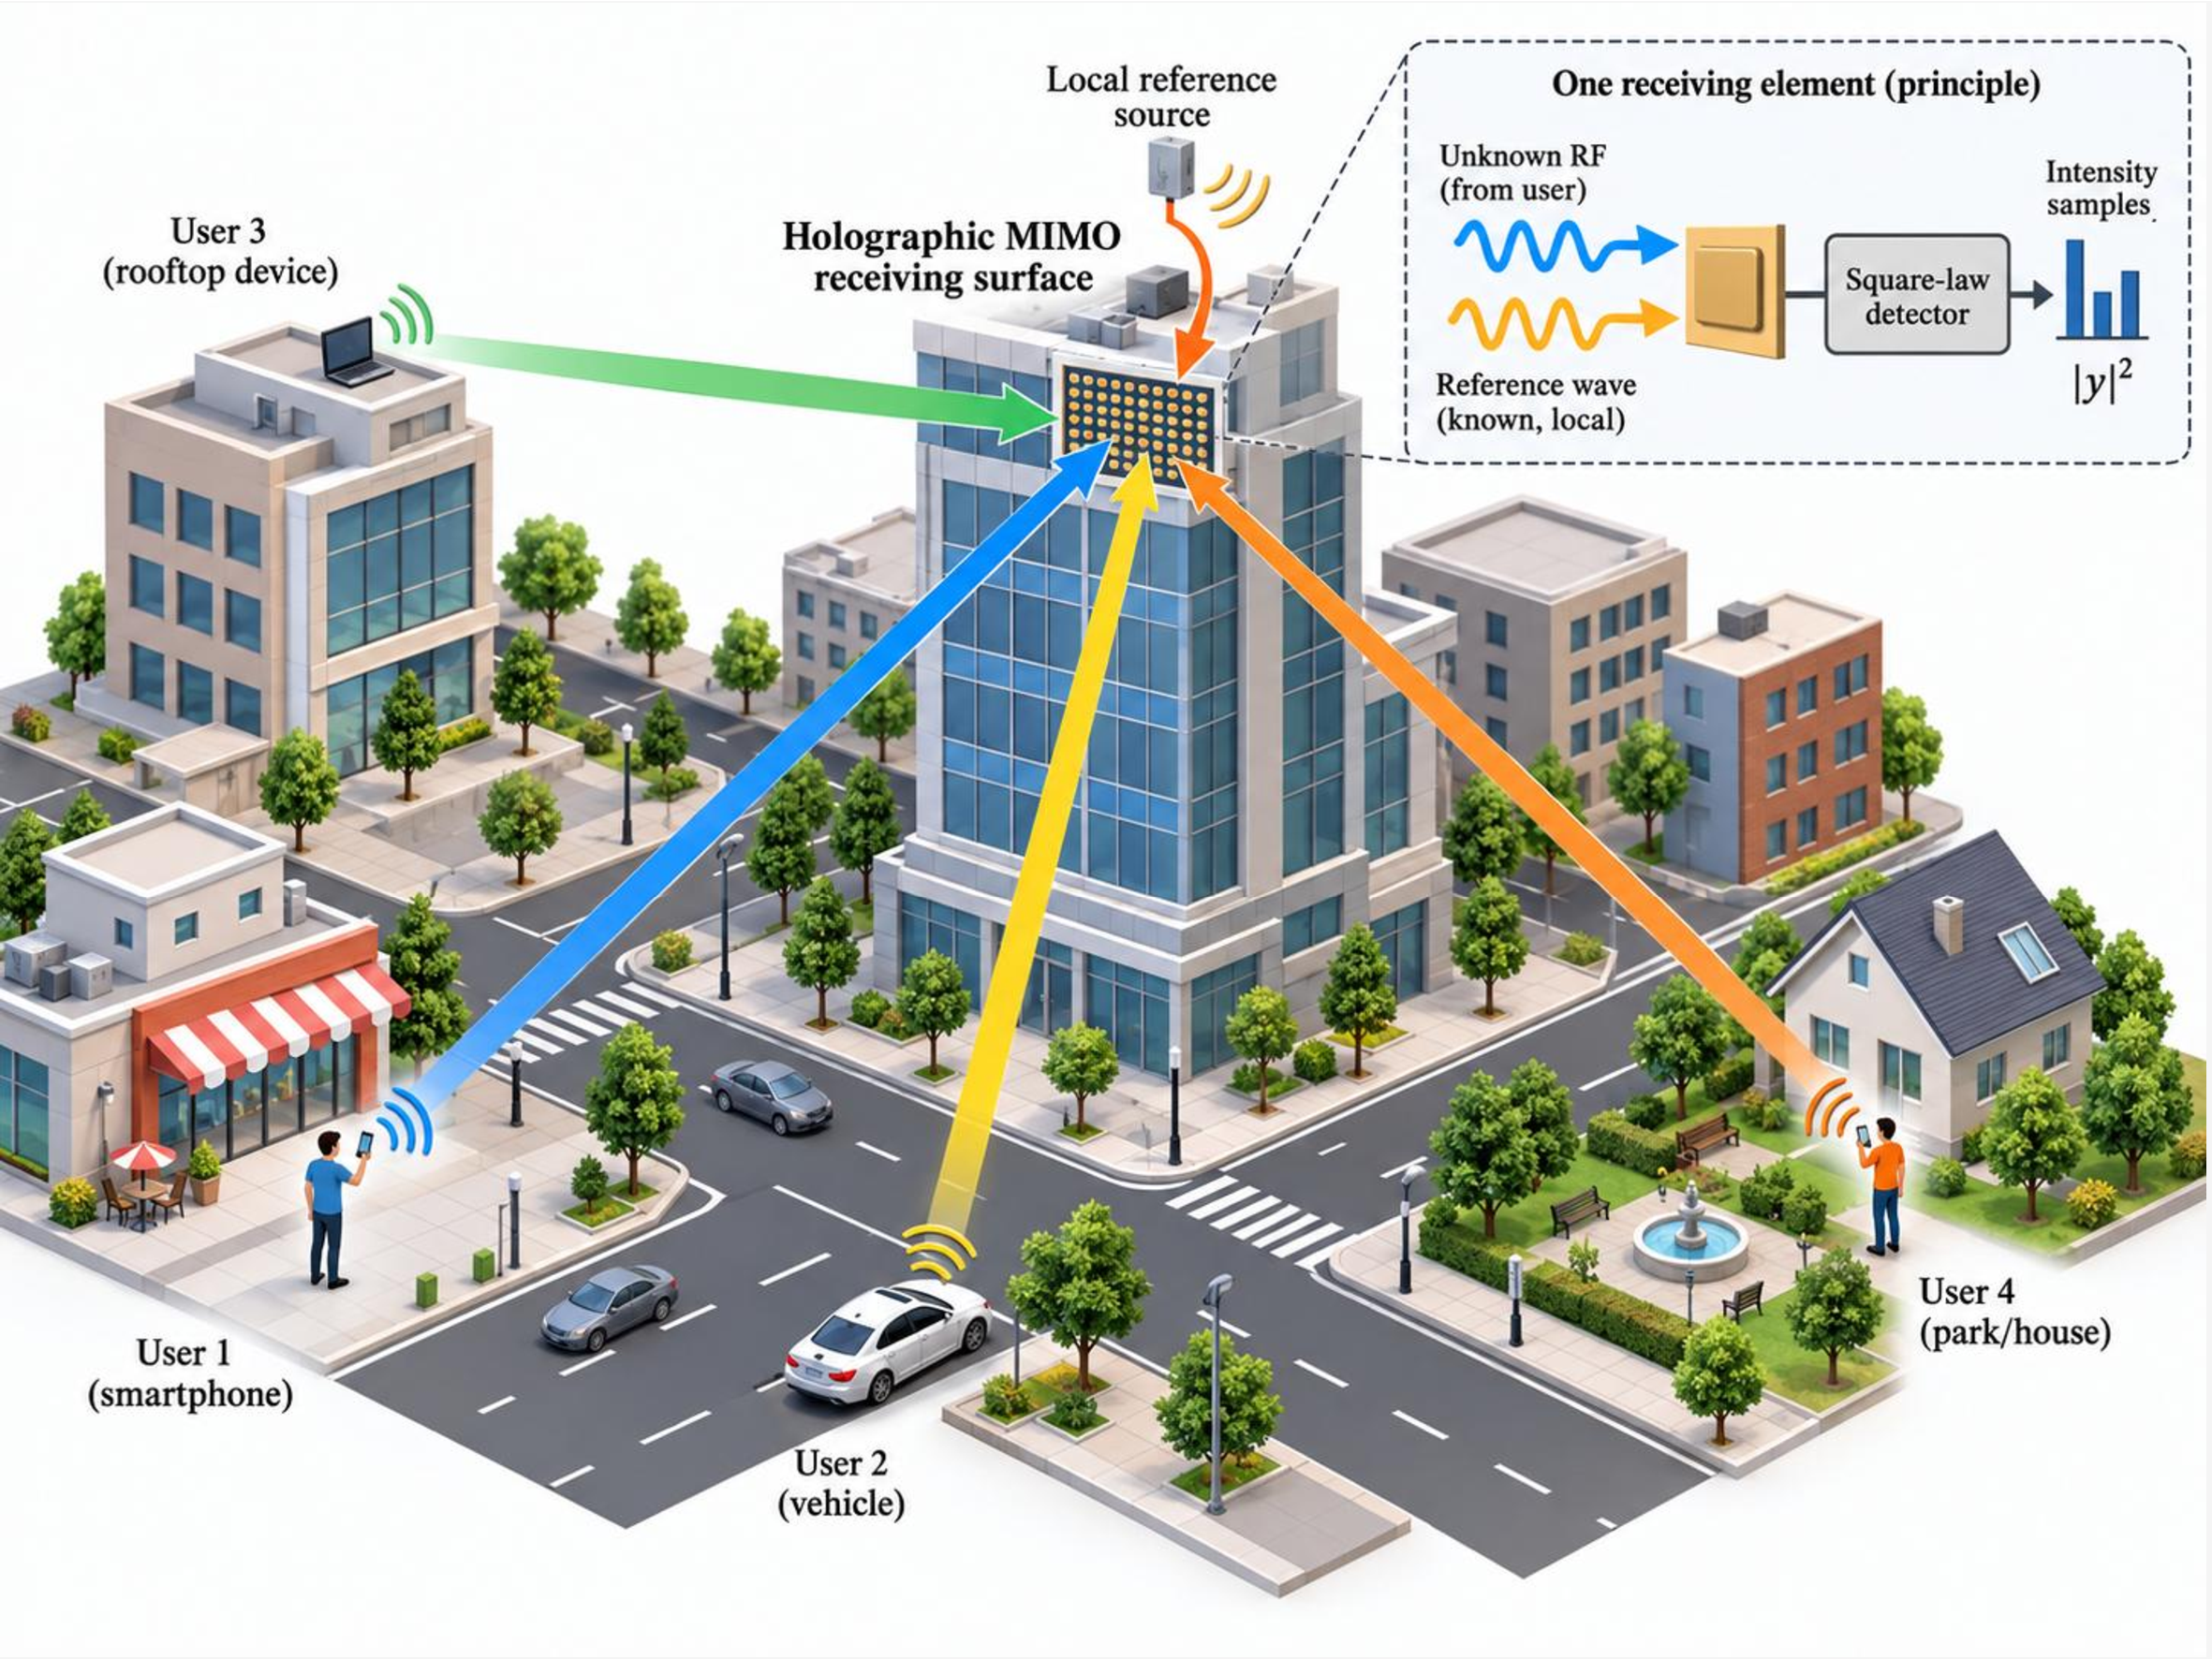
\includegraphics[width=0.95\columnwidth]{images/model/system_modelv1.pdf}
    \caption{Illustration of the proposed multi-user reference-assisted RF holographic reception architecture with intensity-only measurements.}
    \label{fig:model}
\end{figure}

\subsection{Transmitter Model}

The $K$ symbols transmitted by user $l$ in one signaling block are collected in
$\mathbf{s}_l=[s_{l,0},\ldots,s_{l,K-1}]^T\in\mathcal S^K$, where
$\mathcal S=\{c_0,\ldots,c_{M_{\rm mod}-1}\}\subset\mathbb C$ is an
equiprobable constellation normalized to
$\frac{1}{M_{\rm mod}}
\sum_{q=0}^{M_{\rm mod}-1}|c_q|^2
=
\mathbb{E}\{|s_{l,k}|^2\}
=
1$. After pulse
shaping, the complex baseband waveform is
\begin{equation}
x_l(t)
=
\sqrt{P_l}
\sum_{k=0}^{K-1} s_{l,k} p(t-kT_s),
\label{eq:baseband_signal_l}
\end{equation}
Here, $P_l$ is the transmit power, $p(t)$ is the pulse-shaping filter, and
$T_s$ is the symbol duration.
The corresponding real passband waveform radiated by user $l$ is
\begin{equation}
x_l^{\rm RF}(t)
=
\sqrt{2}\operatorname{Re}\!\left\{x_l(t)e^{j2\pi f_ct}\right\},
\label{eq:passband_signal_l}
\end{equation}
where $f_c$ is the carrier frequency. Under the usual carrier-period
averaging, the factor $\sqrt{2}$ makes the average power of
$x_l^{\rm RF}(t)$ equal to the envelope power $|x_l(t)|^2$. Thus, $x_l(t)$
contains the pulse-shaped amplitude and phase information, while the carrier
term translates that waveform to RF for propagation. 

\subsection{Far-Field Channel Model}

The RF holographic receiving surface is modeled as an
$N_y\times N_z$ uniform planar array (UPA) with a total of
$N_{\rm r}=N_yN_z$ receiving elements. 
Without loss of generality, the array is assumed to lie on the $yz$-plane, 
with its geometric center located at the origin. 
The inter-element spacings along the $y$- and $z$-axes are denoted by 
$d_y$ and $d_z$, respectively. 
Accordingly, the position vector of the $(n,m)$-th receiving element is
\begin{equation}
\mathbf r_{n,m}
=
[0,y_n,z_m]^T,
\end{equation}
where $y_n
=
\left(n-\frac{N_y+1}{2}\right)d_y, n=1,\ldots,N_y$, and $z_m
=
\left(m-\frac{N_z+1}{2}\right)d_z, m=1,\ldots,N_z$.
This centered coordinate convention is adopted throughout the paper for
the subsequent far-field array-response modeling. The centered
coordinates introduce no loss of generality because a change of origin produces
only a user-dependent phase that can be absorbed into the complex gain.

Under far-field propagation, user $l$ produces a plane wave with polar angle
$\theta_l$ measured from the array broadside and azimuth angle $\phi_l$ measured
from the positive $y$-axis in the $yz$-plane. With $k_0=2\pi/\lambda$, the
relevant tangential wavenumbers are
$k_{l,y}=k_0\sin\theta_l\cos\phi_l$ and
$k_{l,z}=k_0\sin\theta_l\sin\phi_l$. The phase at element $(n,m)$ is
\begin{equation}
\psi_{n,m}^{(l)}
=
\mathbf{k}_l^T\mathbf{r}_{n,m}
=
k_{l,y}y_n+k_{l,z}z_m.
\label{eq:element_phase_shift}
\end{equation}
The far-field amplitude is taken as constant across the aperture, while path
loss, shadowing, propagation phase, and the residual constant carrier-phase
offset relative to the receiver reference are absorbed into
$\alpha_l\in\mathbb C$. Accordingly,
\begin{equation}
\mathbf{h}_l
=
\alpha_l\mathbf{v}_l,
\qquad
[\mathbf v_l]_{\iota(n,m)}=e^{j\psi_{n,m}^{(l)}},
\label{eq:user_channel_vector}
\end{equation}
where $\iota(n,m)=(n-1)N_z+m$. Collecting all users gives
\begin{equation}
\mathbf{H}
=
[\mathbf h_1,\ldots,\mathbf h_L]
=\underbrace{[\mathbf v_1,\ldots,\mathbf v_L]}_{\mathbf V}
\underbrace{\operatorname{diag}(\alpha_1,\ldots,\alpha_L)}_{\boldsymbol\Gamma}
=\mathbf V\boldsymbol\Gamma,
\label{eq:H_V_Gamma}
\end{equation}
which separates the directional array response from the complex path gains.
The single dominant far-field path per scheduled user is adopted to expose the
DOA-dependent parametric structure targeted by the estimator. More general
wideband or multipath fields remain compatible with the affine intensity
observation model, but require an expanded channel parametrization and are not
considered here.


\subsection{Reference-Assisted Holographic Reception Model}

The element-wise reference signals are derived from a common local oscillator
operating at $f_c$ and distributed across the surface through a power-divider,
RF feed lines, and prescribed phase-delay sections
\cite{huangjd2024CS,yin2025hisprototype}. Thus, all reference branches
share the same carrier and maintain stable relative phases over each detection
interval. Fixed amplitude and phase offsets introduced by the distribution
network are assumed to be calibrated and included in the prescribed reference
coefficients. Let $\mathbf x(t)=[x_1(t),\ldots,x_L(t)]^T$. At receiving unit $i$,
the resulting reference is
\begin{equation}
b_i^{\rm RF}(t)
=
\sqrt{2}\operatorname{Re}\!\left\{b_i e^{j2\pi f_ct}\right\},
\qquad b_i=\rho_i e^{j\chi_i},
\label{eq:rf_reference_wave}
\end{equation}
where $\rho_i$ and $\chi_i$ are its prescribed amplitude and phase. Let
$\mathbf b=[b_1,\ldots,b_{N_{\rm r}}]^T$ collect the reference coefficients.
In the spatial four-phase implementation, distinct receiving units are assigned
$\chi_i\in\{0,\pi/2,\pi,3\pi/2\}$ and operate simultaneously. Hence, the four
phases form a calibrated spatial code across the aperture; they are not four
sequential observations of the same field coordinate and incur no additional
symbol intervals.

Under the narrowband model, the received user field has envelope
$[\mathbf H\mathbf x(t)]_i$. Its superposition with
\eqref{eq:rf_reference_wave} gives
\begin{equation}
r_i^{\rm RF}(t)
=
\sqrt{2}\operatorname{Re}\!\left\{
\left([\mathbf H\mathbf x(t)]_i+b_i\right)e^{j2\pi f_ct}
\right\}.
\label{eq:composite_rf_field}
\end{equation}
Here, $\mathbf H\mathbf x(t)$ contains the propagation response and unknown
user phases, whereas $b_i$ is receiver controlled. The reference-assisted
interference is therefore formed in the analog RF domain before square-law
detection and sampling.

\begin{figure*}[t]
    \centering
    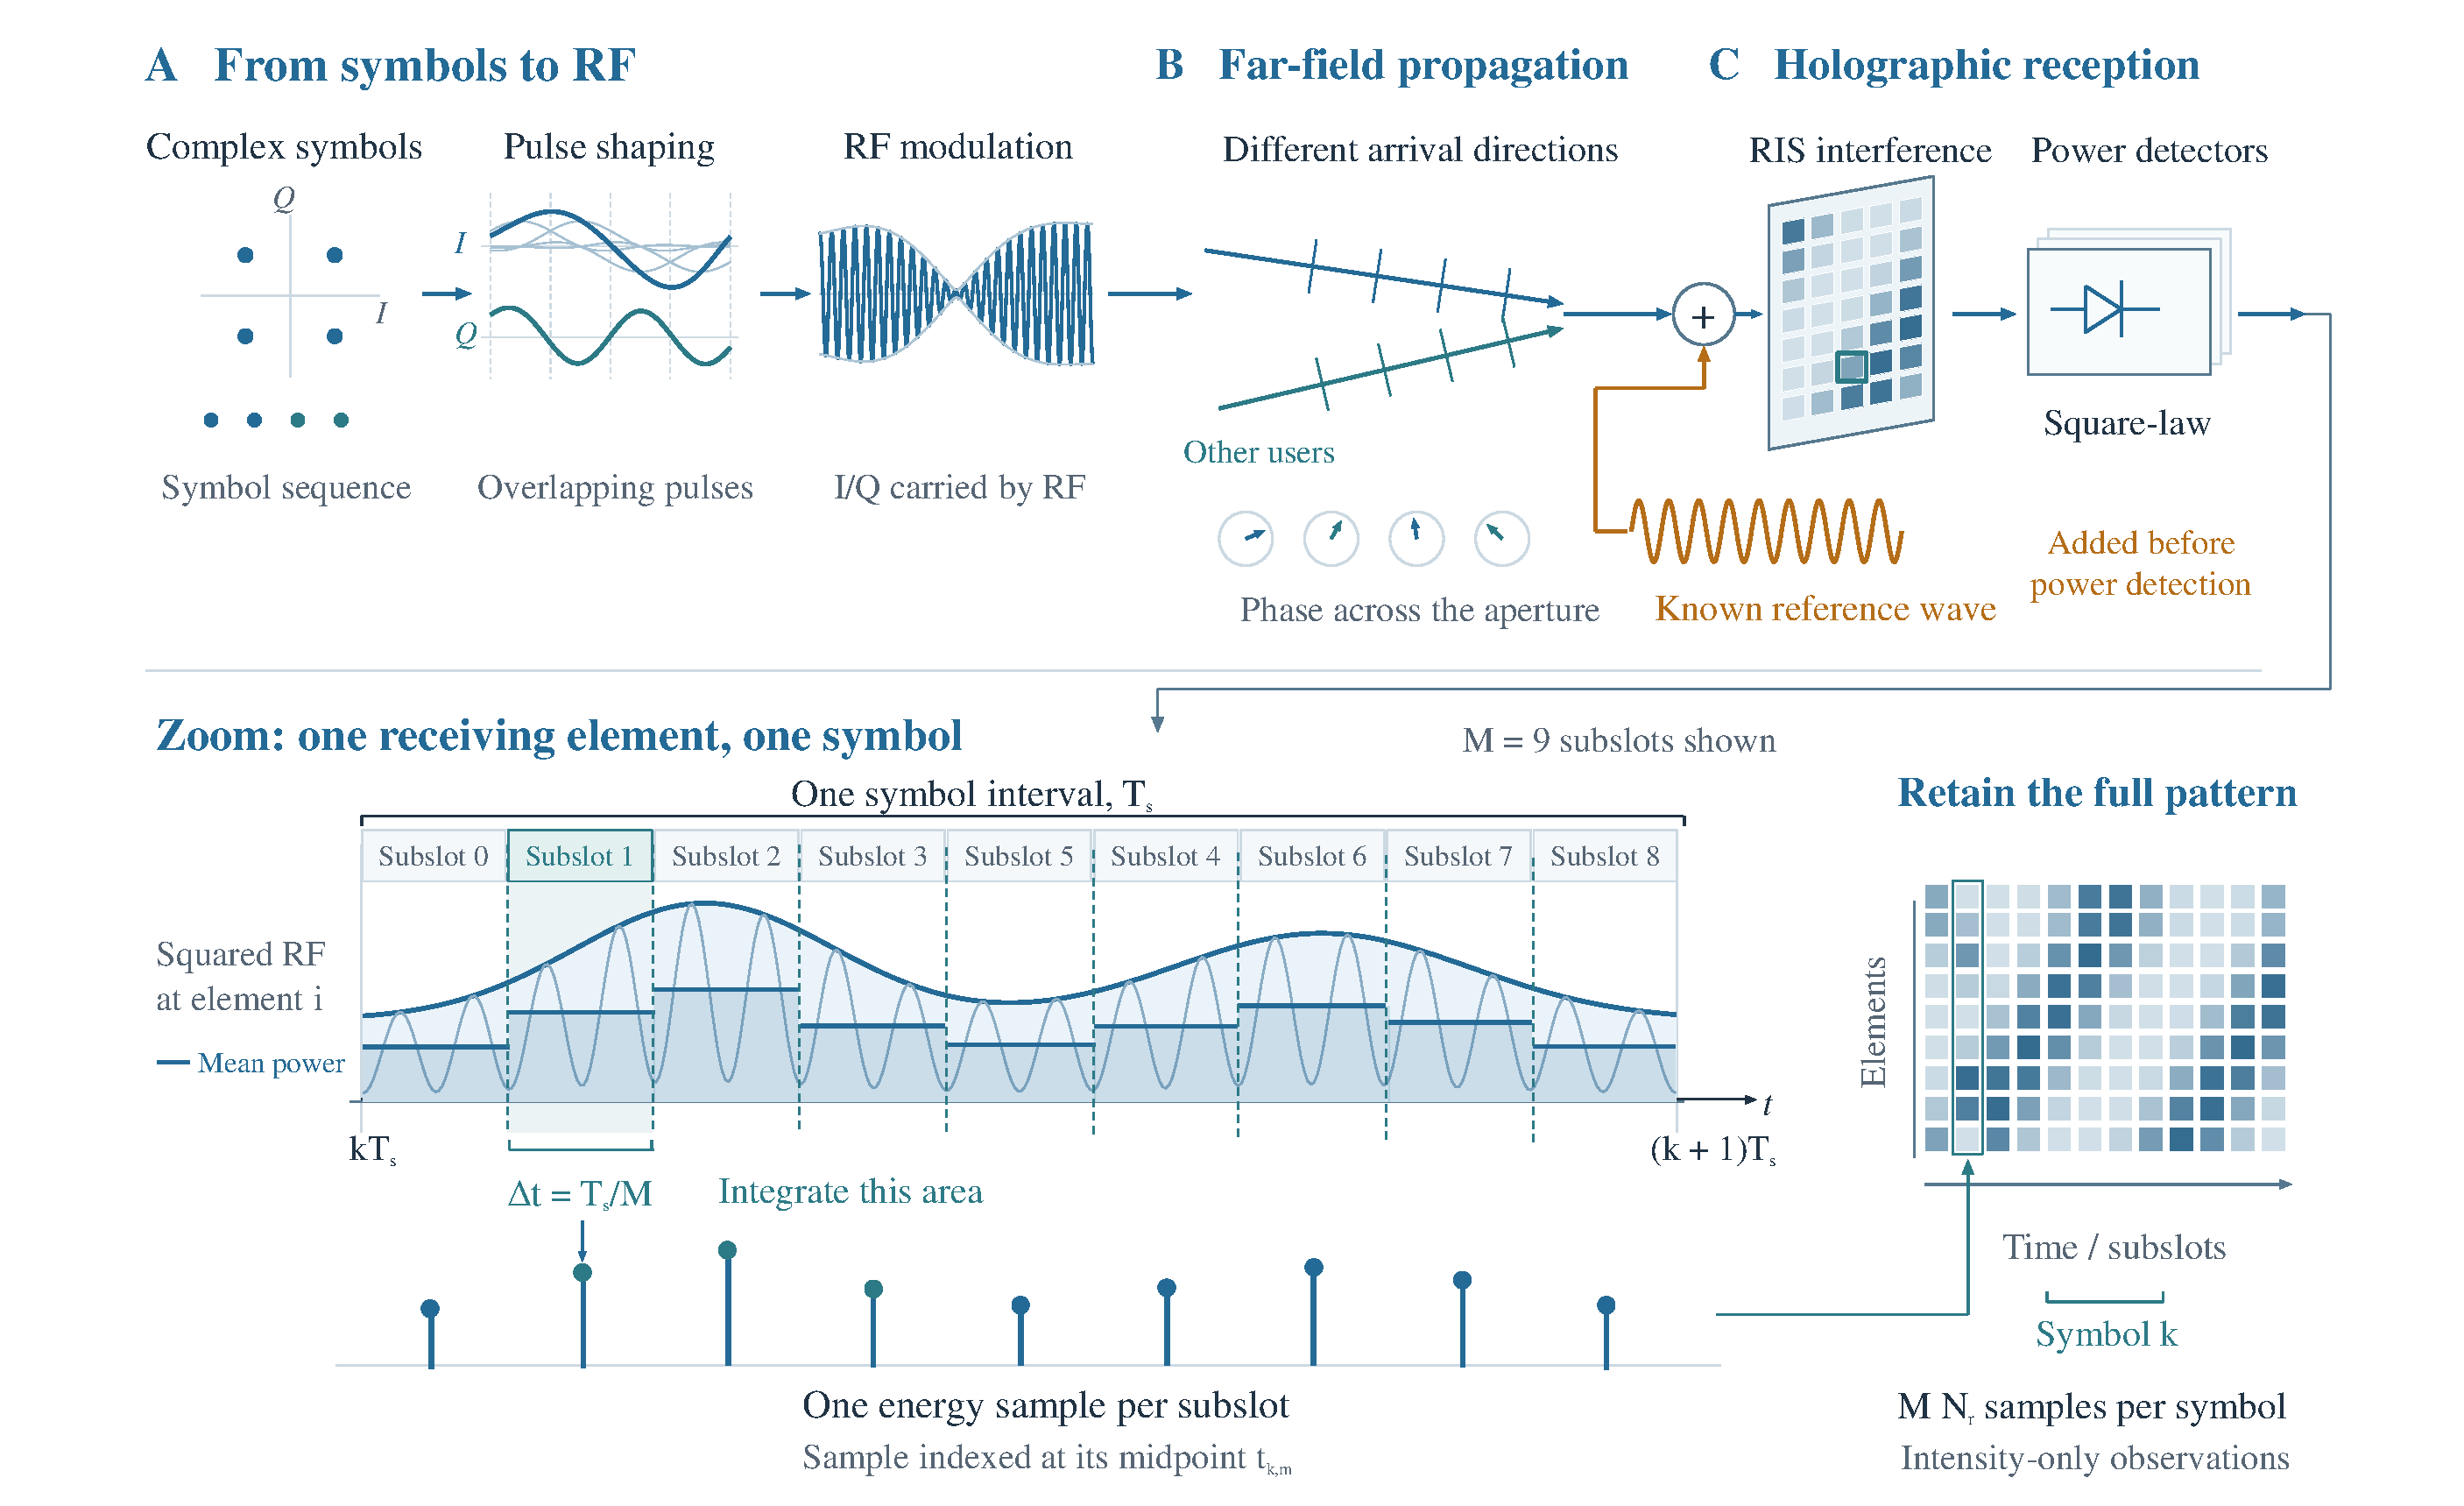
\includegraphics[
        width=0.98\textwidth,
        trim={2cm 0cm 1.8cm 0cm},
        clip
    ]{images/final.pdf}
    \caption{Reference-assisted holographic reception model. 
Finite-alphabet symbols are pulse-shaped and upconverted to RF signals. 
After far-field propagation, the incident fields from different users form direction-dependent phase patterns across the holographic aperture. 
A known reference wave is added at the RF front end before square-law detection, converting relative phase information into intensity variations. 
    When waveform variation within a symbol must be resolved, the symbol interval is divided into $M$ subslots; otherwise, $M=1$. The receiver preserves the resulting spatial intensity pattern for channel estimation and symbol detection.}
    \label{fig:your_figure}
\end{figure*}

Each symbol may be observed over $M$ temporal subslots of duration $\Delta_t=T_s/M$, with
centers $t_{k,m}=kT_s+(m+1/2)\Delta_t$ and intervals
$\mathcal I_{k,m}=[kT_s+m\Delta_t,kT_s+(m+1)\Delta_t)$. Direct square-law
detection and integration are applied to the RF waveform in
\eqref{eq:composite_rf_field}. For compactness, denote its composite complex
envelope by $u_i(t)\triangleq[\mathbf H\mathbf x(t)]_i+b_i$. Then
\begin{equation}
\begin{aligned}
z_i[k,m]
&=\frac{1}{\Delta_t}\int_{\mathcal I_{k,m}}
\bigl[r_i^{\rm RF}(\tau)\bigr]^2d\tau+w_i[k,m]\\
&=\frac{1}{\Delta_t}\int_{\mathcal I_{k,m}}
|u_i(\tau)|^2d\tau\\
&\quad+\frac{1}{\Delta_t}\operatorname{Re}\!\left\{
\int_{\mathcal I_{k,m}}u_i^2(\tau)e^{j4\pi f_c\tau}d\tau
\right\}+w_i[k,m]\\
&\simeq\frac{1}{\Delta_t}\int_{\mathcal I_{k,m}}
|u_i(\tau)|^2d\tau+w_i[k,m].
\end{aligned}
\label{eq:subslot_energy_baseband}
\end{equation}
Thermal and front-end noise physically perturb the incident RF field before
square-law detection. After integration and calibration of the mean noise
floor, its centered contribution appears at the detector output together with
detector and readout imperfections. These aggregate effects are represented by
$w_i[k,m]$, rather than by separate noise terms before and after detection.
Since each subslot averages many RF noise samples, $w_i[k,m]$ is approximated
below as independent zero-mean Gaussian noise with constant variance, yielding
a tractable effective intensity-domain model. An exact pre-detection complex
Gaussian model instead produces signal-dependent noncentral chi-squared
observations and is not pursued here. The second equality follows from
$[\sqrt{2}\operatorname{Re}\{u_i(\tau)e^{j2\pi f_c\tau}\}]^2
=|u_i(\tau)|^2+\operatorname{Re}\{u_i^2(\tau)e^{j4\pi f_c\tau}\}$.
Because $u_i(t)$ varies on the envelope time scale, the oscillatory $2f_c$
term averages out when $\Delta_t f_c\gg1$, yielding the last line. Importantly,
the retained envelope energy satisfies
$|u_i(t)|^2=|[\mathbf H\mathbf x(t)]_i|^2+|b_i|^2
+2\operatorname{Re}\{b_i^*[\mathbf H\mathbf x(t)]_i\}$; hence, integration
removes the carrier-frequency oscillation but preserves the array and symbol
phases through their interference with the known reference. Equation
\eqref{eq:subslot_energy_baseband} is therefore an analytical representation
of the measured RF energy, not coherent downconversion or I/Q sampling. If the
envelope is approximately constant within a subslot, stacking the
$N_{\rm r}$ element outputs yields
\begin{equation}
\mathbf z[k,m]
=
\left|
\mathbf H\mathbf x[k,m]+\mathbf b
\right|^2
+
\mathbf w[k,m]
\in\mathbb R^{N_{\rm r}},
\label{eq:discrete_intensity_measurement}
\end{equation}
where $\mathbf x[k,m]=\mathbf x(t_{k,m})$ and the squared modulus is
element-wise. The $MN_{\rm r}$ samples associated with each symbol are retained
as a vector. Spatial diversity is supplied by the receiving units and their
reference phases, whereas $M>1$ is used only when temporal envelope samples are
needed; it is not the number of reference phases.

To relate these energy samples to the transmitted symbols, define
$\mathbf D_P=\operatorname{diag}(\sqrt{P_1},\ldots,\sqrt{P_L})$,
$[\mathbf P]_{kM+m,j}=p(t_{k,m}-jT_s)$, and stack
$\mathbf s=[\mathbf s_1^T,\ldots,\mathbf s_L^T]^T$. The matrix
$\mathbf P_{\rm tx}\triangleq\mathbf D_P\otimes\mathbf P\in
\mathbb C^{LKM\times LK}$ maps $\mathbf s$ to the sampled user envelopes,
where $\otimes$ denotes the Kronecker product.

For general pulse shaping, neighboring symbols may overlap, so the
$KMN_{\rm r}$ measurements must be processed jointly. Let $\boldsymbol\Pi$
reorder the user-major envelope $\mathbf P_{\rm tx}\mathbf s$ into
time-major form. Stacking \eqref{eq:discrete_intensity_measurement} over all
subslots then yields the compact block-level model
\begin{equation}
\mathbf z=|\mathbf G\mathbf s+\mathbf b_{\rm eq}|^2+\mathbf w,
\label{eq:block_level_intensity_model}
\end{equation}
where $\mathbf G\triangleq(\mathbf I_{KM}\otimes\mathbf H)
\boldsymbol\Pi\mathbf P_{\rm tx}\in\mathbb C^{KMN_{\rm r}\times LK}$ and
$\mathbf b_{\rm eq}\triangleq\mathbf 1_{KM}\otimes\mathbf b$. Thus,
$\mathbf s\in\mathcal S^{LK}$ and
$\mathbf z,\mathbf w\in\mathbb R^{KMN_{\rm r}}$. When intersymbol overlap is
negligible, \eqref{eq:block_level_intensity_model} separates into symbol-wise
models; otherwise, it describes joint block detection.

\subsection{Two-Phase Transmission Protocol and Unified Observation Model}

The receiver uses a training phase to estimate the channel from known pilots and
a data phase to detect finite-alphabet symbols using the estimated channel. Both
phases follow \eqref{eq:block_level_intensity_model}, but their unknowns have
different structures.

\subsubsection{Training Phase}

Let $\mathbf x_{\rm p}[t]\in\mathbb C^L$ be the known waveform in pilot
subslot $t=0,\ldots,T_{\rm p}-1$, and define
$\mathbf h=\operatorname{vec}(\mathbf H)$. Stacking the element-wise
observations and using
$\mathbf H\mathbf x_{\rm p}[t]=(\mathbf x_{\rm p}^T[t]\otimes
\mathbf I_{N_{\rm r}})\mathbf h$ gives
\begin{equation}
\mathbf{z}_{\rm p}
=
\left|
\mathbf{G}_{\rm p}\mathbf{h}
+
\mathbf{b}_{\rm p}
\right|^2
+
\mathbf{w}_{\rm p},
\label{eq:block_pilot_phase_model}
\end{equation}
where $\mathbf G_{\rm p}$ stacks
$\mathbf x_{\rm p}^T[t]\otimes\mathbf I_{N_{\rm r}}$, and
$\mathbf b_{\rm p}$ and $\mathbf w_{\rm p}$ stack the reference and noise. For
the fixed spatial code considered here, $\mathbf b_{\rm p}$ repeats the same
calibrated $N_{\rm r}$-entry phase map at every pilot time.
The far-field structure in \eqref{eq:H_V_Gamma} will later reduce the unknown
from the full vector $\mathbf h$ to the DOAs and complex path gains.

\subsubsection{Data Transmission Phase}

For a data block of $K_{\rm d}$ symbols per user, let
$\mathbf s_{\rm d}\in\mathcal S^{LK_{\rm d}}$ denote the stacked symbol
vector. Denote the true noiseless response by
$\boldsymbol\mu_{\rm d}(\mathbf s;\mathbf H)
\triangleq|\mathbf G_{\rm d}(\mathbf H)\mathbf s+
\mathbf b_{\rm d}|^2$. Using $\widehat{\mathbf H}$, the receiver
forms the detection template
$\widehat{\boldsymbol\mu}_{\rm d}(\mathbf s)
\triangleq|\mathbf G_{\rm d}(\widehat{\mathbf H})\mathbf s+
\widehat{\mathbf b}_{\rm d}|^2$. The actual observation can therefore be
written as
\begin{equation}
\mathbf{z}_{\rm d}
=
\widehat{\boldsymbol\mu}_{\rm d}(\mathbf s_{\rm d})
+\mathbf e_{\rm CSI}(\mathbf s_{\rm d})
+
\mathbf{w}_{\rm d},
\label{eq:block_data_phase_model}
\end{equation}
where $\mathbf e_{\rm CSI}(\mathbf s)\triangleq
\boldsymbol\mu_{\rm d}(\mathbf s;\mathbf H)-
\widehat{\boldsymbol\mu}_{\rm d}(\mathbf s)$ is the generally
symbol-dependent CSI-mismatch error and vanishes for perfect CSI. Here,
$Q_{\rm d}=N_{\rm r}MK_{\rm d}$, and $\widehat{\mathbf b}_{\rm d}=\mathbf b_{\rm d}$
is the calibrated receiver reference. Thus, the training and data phases share
the same affine intensity structure, but the latter performs finite-alphabet
detection with an estimated observation map.


\section{Uniqueness and Stability of Reference-Assisted Energy Detection}
\label{sec:uniqueness_stability}

Reliable recovery from intensity-only measurements requires more than the
existence of a solution: distinct channels or symbol vectors must produce
distinct energy observations, and small measurement perturbations must not
cause arbitrarily large reconstruction errors. These requirements are captured
by uniqueness and stability, respectively, and are fundamental to determining
whether the reference wave and spatial sampling provide sufficient information.
Exploiting the quadratic structure of the reference-assisted energy mapping, we
establish an exact secant-based uniqueness condition and derive lower and upper
Lipschitz bounds that quantify robustness. The resulting framework applies to
both continuous channel estimation and finite-alphabet symbol detection.

\subsection{Unified Affine Phase-Retrieval Model}

The training- and data-phase observations derived in Section~II share the form
\begin{equation}
\mathbf z
=
\mathcal T_{\mathbf G,\mathbf b}(\boldsymbol\theta)+\mathbf w,
\qquad
\mathcal T_{\mathbf G,\mathbf b}(\boldsymbol\theta)
\triangleq
\left|\mathbf G\boldsymbol\theta+\mathbf b\right|^2 ,
\label{eq:unified_pr_model}
\end{equation}
where $Q$ is the total number of scalar intensity observations, $D$ is the
complex dimension of the unknown vector, $\mathbf G\in\mathbb C^{Q\times D}$,
$\boldsymbol\theta\in\mathcal X\subseteq\mathbb C^D$,
$\mathbf b\in\mathbb C^Q$, and $\mathbf z,\mathbf w\in\mathbb R^Q$.
Here, $\mathcal X$ denotes the feasible set of the unknown parameter, and the
modulus and square are applied element-wise.  This is an affine
phase-retrieval model \cite{affine_phase_retrieval}.  For full-channel
estimation in the training phase,
$\boldsymbol\theta=\mathbf h=\operatorname{vec}(\mathbf H)$,
$Q=N_{\rm r}T_{\rm p}$, and $D=N_{\rm r}L$.  If the channel is represented by
a lower-dimensional linear complex parameter, $D$ is replaced by the
dimension of that parameter.  In the data phase,
$\boldsymbol\theta=\mathbf s_{\rm d}\in\mathcal S^{LK_{\rm d}}$,
$Q=Q_{\rm d}$, and $D=LK_{\rm d}$.

The reference changes the ambiguity class fundamentally. If $\mathbf b=0$,
$\mathcal T_{\mathbf G,\mathbf 0}(e^{j\varphi}\boldsymbol\theta)
=\mathcal T_{\mathbf G,\mathbf 0}(\boldsymbol\theta)$, so uniqueness is defined
only modulo a global phase. If $\mathbf b\ne0$, the expansion
\begin{equation}
\mathcal T_{\mathbf G,\mathbf b}(\boldsymbol\theta)
=|\mathbf G\boldsymbol\theta|^2+|\mathbf b|^2
+2\operatorname{Re}\{\mathbf b^*\odot\mathbf G\boldsymbol\theta\}
\label{eq:reference_expansion}
\end{equation}
contains phase-sensitive interference, so absolute uniqueness on $\mathcal X$
becomes possible.  A nonzero reference is not sufficient by itself, however:
its phases must probe every feasible field difference in nondegenerate real
directions.

For $\boldsymbol\theta\in\mathbb C^D$, define the realification
$\boldsymbol\theta_{\mathbb R}=[\operatorname{Re}\{\boldsymbol\theta\}^T,
\operatorname{Im}\{\boldsymbol\theta\}^T]^T\in\mathbb R^{2D}$. For two
distinct parameters, define the energy-domain distance
\begin{equation}
d_E(\boldsymbol\theta_1,\boldsymbol\theta_2)
\triangleq
\left\|
\mathcal T_{\mathbf G,\mathbf b}(\boldsymbol\theta_1)
-
\mathcal T_{\mathbf G,\mathbf b}(\boldsymbol\theta_2)
\right\|_2 .
\label{eq:energy_domain_distance_general}
\end{equation}
The optimal lower and upper stability bounds on $\mathcal X$ are
\begin{align}
\alpha_{\mathcal X}
&\triangleq
\inf_{\substack{\boldsymbol\theta_1,\boldsymbol\theta_2\in\mathcal X\\
\boldsymbol\theta_1\ne\boldsymbol\theta_2}}
\frac{d_E(\boldsymbol\theta_1,\boldsymbol\theta_2)}
{\|\boldsymbol\theta_1-\boldsymbol\theta_2\|_2},
\label{eq:lower_stability_constant}\\
\beta_{\mathcal X}
&\triangleq
\sup_{\substack{\boldsymbol\theta_1,\boldsymbol\theta_2\in\mathcal X\\
\boldsymbol\theta_1\ne\boldsymbol\theta_2}}
\frac{d_E(\boldsymbol\theta_1,\boldsymbol\theta_2)}
{\|\boldsymbol\theta_1-\boldsymbol\theta_2\|_2}.
\label{eq:upper_stability_constant}
\end{align}
Thus, the inverse problem is globally stable on $\mathcal X$ if
$0<\alpha_{\mathcal X}\leq\beta_{\mathcal X}<\infty$.  The lower bound is the
important one: it excludes pairs that are far apart in parameter space but
arbitrarily close in energy space.

\subsection{Exact Secant Identity and Global Uniqueness}

The quadratic structure of \eqref{eq:unified_pr_model} gives an exact identity,
which is stronger than a first-order approximation.  For a point
$\boldsymbol\vartheta\in\mathbb C^D$, define the real Jacobian
\begin{equation}
\begin{split}
\mathbf J(\boldsymbol\vartheta)
\triangleq 2\big[&
\operatorname{Re}\{\operatorname{diag}[
(\mathbf G\boldsymbol\vartheta+\mathbf b)^*]\mathbf G\},\\
&-\operatorname{Im}\{\operatorname{diag}[
(\mathbf G\boldsymbol\vartheta+\mathbf b)^*]\mathbf G\}
\big]\in\mathbb R^{Q\times 2D}.
\end{split}
\label{eq:real_jacobian}
\end{equation}

\begin{theorem}[Exact secant identity and pairwise uniqueness]
\label{thm:exact_secant_uniqueness}
For any $\boldsymbol\theta_1,\boldsymbol\theta_2\in\mathbb C^D$, let
$\boldsymbol\mu=(\boldsymbol\theta_1+\boldsymbol\theta_2)/2$ and
$\boldsymbol\delta=\boldsymbol\theta_1-\boldsymbol\theta_2$.  Then
\begin{equation}
\mathcal T_{\mathbf G,\mathbf b}(\boldsymbol\theta_1)
-
\mathcal T_{\mathbf G,\mathbf b}(\boldsymbol\theta_2)
=
\mathbf J(\boldsymbol\mu)\boldsymbol\delta_{\mathbb R}.
\label{eq:exact_secant_identity}
\end{equation}
Consequently, the mapping $\mathcal T_{\mathbf G,\mathbf b}$ is injective on
$\mathcal X$ if and only if, for every distinct
$\boldsymbol\theta_1,\boldsymbol\theta_2\in\mathcal X$,
\begin{equation}
\mathbf J\!\left(
\frac{\boldsymbol\theta_1+\boldsymbol\theta_2}{2}
\right)
(\boldsymbol\theta_1-\boldsymbol\theta_2)_{\mathbb R}
\ne\mathbf0 .
\label{eq:pairwise_ambiguity_condition_main}
\end{equation}
\end{theorem}
\begin{proof}
Applying $|a|^2-|c|^2=\operatorname{Re}\{(a+c)^*(a-c)\}$
element-wise gives
$\operatorname{Re}\{[\mathbf G(\boldsymbol\theta_1+\boldsymbol\theta_2)
+2\mathbf b]^*\odot\mathbf G(\boldsymbol\theta_1-\boldsymbol\theta_2)\}$,
which equals \eqref{eq:exact_secant_identity} after realification.  Hence, two
feasible points have identical intensity observations exactly when the
right-hand side of \eqref{eq:exact_secant_identity} vanishes.  Excluding this
possibility for every distinct pair is therefore equivalent to injectivity on
$\mathcal X$, proving \eqref{eq:pairwise_ambiguity_condition_main}.
\end{proof}

For a full-dimensional continuous set, $\operatorname{rank}(\mathbf G)=D$ is
necessary but not sufficient: a nonzero field difference can still vanish
after the reference-dependent real projection. A sharper conclusion is
available for finite hypotheses.

\begin{corollary}[Generic-reference uniqueness for finite hypotheses]
\label{cor:generic_reference_finite_hypotheses}
Let $\Xi=\{\xi_1,\ldots,\xi_M\}$ be finite, with pre-reference field codewords
$\mathbf u_i=\mathbf f(\xi_i)\in\mathbb C^Q$. For $i\ne j$, set
$\mathbf d_{ij}=\mathbf u_i-\mathbf u_j$ and
$\mathbf a_{ij}=(|\mathbf u_i|^2-|\mathbf u_j|^2)/2$. A pair with
$\mathbf d_{ij}=\mathbf0$ is indistinguishable for every reference; otherwise,
its ambiguous references form the proper real affine set
\begin{equation}
\mathcal B_{ij}^{\rm bad}
=
\left\{
\mathbf b\in\mathbb C^Q:
\operatorname{Re}\{\mathbf b^*\odot\mathbf d_{ij}\}
=-\mathbf a_{ij}
\right\}.
\label{eq:bad_reference_affine_set}
\end{equation}
If all field codewords are distinct, the finite union
$\bigcup_{i<j}\mathcal B_{ij}^{\rm bad}$ has measure zero in $\mathbb C^Q$;
hence, an absolutely continuously distributed reference makes
$|\mathbf u_i+\mathbf b|^2$ pairwise distinct with probability one.
\end{corollary}
\begin{proof}
For two hypotheses in the affine field model, let
$\boldsymbol\mu_{ij}=(\boldsymbol\theta_i+\boldsymbol\theta_j)/2$ and
$\boldsymbol\delta_{ij}=\boldsymbol\theta_i-\boldsymbol\theta_j$, so that
$\mathbf u_i=\mathbf G\boldsymbol\theta_i$,
$\mathbf u_j=\mathbf G\boldsymbol\theta_j$, and
$\mathbf d_{ij}=\mathbf G\boldsymbol\delta_{ij}$.  Expanding the Jacobian--secant
product in \eqref{eq:pairwise_ambiguity_condition_main} gives
\begin{align*}
&\mathbf J(\boldsymbol\mu_{ij})
(\boldsymbol\delta_{ij})_{\mathbb R} \\
&=2\operatorname{Re}\!\left\{
\left(\frac{\mathbf u_i+\mathbf u_j}{2}+\mathbf b\right)^*
\odot(\mathbf u_i-\mathbf u_j)\right\} \\
&=\operatorname{Re}\!\left\{(\mathbf u_i+\mathbf u_j)^*
\odot\mathbf d_{ij}\right\}
+2\operatorname{Re}\!\left\{\mathbf b^*\odot\mathbf d_{ij}\right\} \\
&=|\mathbf u_i|^2-|\mathbf u_j|^2
+2\operatorname{Re}\!\left\{\mathbf b^*\odot\mathbf d_{ij}\right\} \\
&=2\left(\mathbf a_{ij}
+\operatorname{Re}\!\left\{\mathbf b^*\odot\mathbf d_{ij}\right\}\right).
\end{align*}
The cross terms in the third line cancel after taking the real part.  Hence,
the pair is ambiguous precisely when
$\operatorname{Re}\{\mathbf b^*\odot\mathbf d_{ij}\}=-\mathbf a_{ij}$,
which proves \eqref{eq:bad_reference_affine_set}.  This final identity depends
only on the two field codewords and therefore also holds for a general finite
mapping $\mathbf f$.

If $d_{ij,q}=0$, then $u_{i,q}=u_{j,q}$ and $a_{ij,q}=0$, so that coordinate
imposes no restriction.  If $d_{ij,q}\ne0$, all ambiguous reference values are
\begin{equation*}
b_q=\left(-\frac{a_{ij,q}}{|d_{ij,q}|^2}+j\tau_q\right)d_{ij,q},
\qquad \tau_q\in\mathbb R,
\end{equation*}
which is one real affine constraint in $\mathbb C$.  Therefore, if
$r_{ij}=|\{q:d_{ij,q}\ne0\}|\geq1$, then
$\mathcal B_{ij}^{\rm bad}$ has real dimension $2Q-r_{ij}<2Q$ and hence
Lebesgue measure zero.  A finite union of such sets remains measure zero,
establishing the almost-sure uniqueness claim.
\end{proof}

For $b_q=\rho_qe^{j\chi_q}$, an active coordinate is ambiguous only when
$\rho_q|d_{ij,q}|\cos(\angle d_{ij,q}-\chi_q)=-a_{ij,q}$, which excludes at
most two phases. Continuous phases are therefore ambiguity-free almost surely
when the reference support meets every field difference. This almost-sure
statement relies on continuous phase variation and does not extend directly to
a fixed or spatially coupled finite-phase code, which must instead be checked
using \eqref{eq:bad_reference_affine_set} or its actual minimum distance. For
$\mathbf f(\boldsymbol\theta)=\mathbf G\boldsymbol\theta$,
the premise reduces to
$\mathbf G(\boldsymbol\theta_i-\boldsymbol\theta_j)\ne\mathbf0$. Full column
rank is sufficient but unnecessary on a finite set, while a difference already
annihilated by $\mathbf G$ cannot be restored by any reference. The result also
applies to $\mathbf u_i=\mathbf g_{\rm p}(\boldsymbol\eta_i)$ on a finite
angular grid when its nuisance parameters are fixed or discretized; continuous
gains require the parametric analysis below.

Generic injectivity on a finite set does not by itself ensure a useful noise
margin. Returning to a general feasible set, let
$\mathcal M_{\mathcal X}=\{(\boldsymbol\theta_1+
\boldsymbol\theta_2)/2:\boldsymbol\theta_1,\boldsymbol\theta_2\in
\mathcal X\}$ be the midpoint set. The exact identity yields computable
two-sided bounds.

\begin{theorem}[Jacobian stability bounds]
\label{thm:jacobian_bounds}
Define
\begin{equation}
\underline\sigma_J
\triangleq\inf_{\boldsymbol\mu\in\mathcal M_{\mathcal X}}
\sigma_{\min}(\mathbf J(\boldsymbol\mu)),\qquad
\overline\sigma_J
\triangleq\sup_{\boldsymbol\mu\in\mathcal M_{\mathcal X}}
\sigma_{\max}(\mathbf J(\boldsymbol\mu)).
\end{equation}
Then
\begin{equation}
\underline\sigma_J\,
\|\boldsymbol\theta_1-\boldsymbol\theta_2\|_2
\le d_E(\boldsymbol\theta_1,\boldsymbol\theta_2)
\le
\overline\sigma_J\,
\|\boldsymbol\theta_1-\boldsymbol\theta_2\|_2
\label{eq:global_bilipschitz_bounds}
\end{equation}
for all pairs in $\mathcal X$. Consequently,
$\alpha_{\mathcal X}\ge\underline\sigma_J$ and
$\beta_{\mathcal X}\le\overline\sigma_J$.
\end{theorem}
\begin{proof}
Apply the singular-value inequalities to
\eqref{eq:exact_secant_identity} over the midpoint set.
\end{proof}

The bound $\underline\sigma_J>0$ is a convenient sufficient condition for
global stability, but it can be conservative because it tests every direction
at every midpoint, including directions that may not connect two feasible
points.  The exact constant in \eqref{eq:lower_stability_constant}, or
equivalently the restricted secants in \eqref{eq:exact_secant_identity}, is the
sharp criterion.

The stability constants also depend on the balance between the received field
and the reference wave.  To make this dependence explicit, let
$u_q(\boldsymbol\theta)=[\mathbf G\boldsymbol\theta]_q$ and, whenever
$u_q(\boldsymbol\theta)\ne0$, define the per-measurement reference-to-signal
energy ratio and the corresponding normalized interference depth as
\begin{equation}
\gamma_q(\boldsymbol\theta)
\triangleq\frac{|b_q|^2}{|u_q(\boldsymbol\theta)|^2},\qquad
\kappa_q(\boldsymbol\theta)
\triangleq\frac{2\sqrt{\gamma_q(\boldsymbol\theta)}}
{1+\gamma_q(\boldsymbol\theta)}.
\label{eq:reference_signal_energy_balance}
\end{equation}
Writing $\Delta\phi_q=\angle u_q-\angle b_q$, the $q$th noiseless
measurement becomes
\begin{equation}
[\mathcal T_{\mathbf G,\mathbf b}(\boldsymbol\theta)]_q
=\bigl(|u_q|^2+|b_q|^2\bigr)
\bigl[1+\kappa_q(\boldsymbol\theta)\cos(\Delta\phi_q)\bigr].
\label{eq:normalized_reference_interference}
\end{equation}
Here $0\leq\kappa_q\leq1$, with its maximum attained when the two incident
fields have equal energy.  It approaches zero when either field dominates,
showing that the phase-sensitive interference then occupies only a small
fraction of the detected energy.

More directly, consider the global-phase perturbation
$e^{j\varphi}\boldsymbol\theta$.  Its tangent direction satisfies
\begin{equation}
\begin{aligned}
\mathbf J(\boldsymbol\theta)(j\boldsymbol\theta)_{\mathbb R}
&=-2\operatorname{Im}\{\mathbf b^*\odot\mathbf G\boldsymbol\theta\},\\
\sigma_{\min}(\mathbf J(\boldsymbol\theta))
&\leq
\frac{2\|\operatorname{Im}\{\mathbf b^*\odot
\mathbf G\boldsymbol\theta\}\|_2}{\|\boldsymbol\theta\|_2}.
\end{aligned}
\label{eq:reference_phase_direction_sensitivity}
\end{equation}
Equation~\eqref{eq:reference_phase_direction_sensitivity} shows that a
vanishing reference restores the global-phase ambiguity, while energy balance
alone is insufficient because phase-aligned samples remain insensitive.
Reference strength and phase diversity must therefore be designed jointly and
assessed through $\underline\sigma_J$.  These bounds are understood on the
bounded gain-and-power region of interest: affine phase retrievability is
bi-Lipschitz on compact feasible sets, but not uniformly so over the entire
unbounded space \cite[Theorem~4.1, Proposition~4.1]{affine_phase_retrieval}.

\subsection{Parametric Channel Uniqueness Requirements}
\label{subsec:parametric_channel_uniqueness}

The affine phase-retrieval result in \cite[Theorem~3.1]{affine_phase_retrieval}
states that a mapping on $\mathbb C^D$ is globally injective if and only if its
real Jacobian has rank $2D$ at every point.  For unstructured channel training,
$D_h=N_{\rm r}L$, $Q_{\rm p}=N_{\rm r}T_{\rm p}$, and the unknown is
$\mathbf h=\operatorname{vec}(\mathbf H)\in\mathbb C^{D_h}$.  The universal
minimum-measurement result in \cite[Theorem~3.2]{affine_phase_retrieval}
therefore gives the necessary condition
\begin{equation}
Q_{\rm p}=N_{\rm r}T_{\rm p}\geq3D_h=3N_{\rm r}L
\quad\Longrightarrow\quad T_{\rm p}\geq3L.
\label{eq:unstructured_global_measurement_count}
\end{equation}
This bound concerns global recovery over the entire space
$\mathbb C^{N_{\rm r}L}$; hence, increasing $N_{\rm r}$ does not reduce the
required number of pilot subslots because it increases the number of unknown
channel coefficients by the same factor.  A generic unconstrained affine
measurement pair is sufficient when $Q_{\rm p}\geq4D_h-1$
\cite[Theorem~3.4]{affine_phase_retrieval}.  This generic result is only a
benchmark here, however, because
$\mathbf G_{\rm p}=\mathbf X_{\rm p}\otimes\mathbf I_{N_{\rm r}}$ has a
structured Kronecker form.

The far-field model reduces the channel to a real parameter manifold.  Let
$d_{\rm a}$ be the number of angular parameters per user and define
$p=(d_{\rm a}+2)L$, where the additional two parameters are the real and
imaginary parts of each path gain.  With
$\mathbf h_{\mathbb R}(\boldsymbol\eta)\triangleq
[\operatorname{Re}\{\mathbf h(\boldsymbol\eta)\}^{T},
\operatorname{Im}\{\mathbf h(\boldsymbol\eta)\}^{T}]^{T}$ and
$\mathbf H_{\eta}\triangleq
\partial\mathbf h_{\mathbb R}/\partial\boldsymbol\eta^{T}$, the chain rule
gives the parameter-domain Jacobian
\begin{equation}
\mathbf J_{\eta}(\boldsymbol\eta)
=
\mathbf J_h(\mathbf h(\boldsymbol\eta))\mathbf H_{\eta}(\boldsymbol\eta)
\in\mathbb R^{Q_{\rm p}\times p},
\label{eq:parametric_jacobian_chain_rule}
\end{equation}
where $\mathbf J_h$ is \eqref{eq:real_jacobian} evaluated with
$\mathbf G=\mathbf G_{\rm p}$ and $\mathbf b=\mathbf b_{\rm p}$.
If each of the $K_{\rm p}$ pilot symbols is observed over $M$ subslots, then
$T_{\rm p}=MK_{\rm p}$.

\begin{corollary}[Parametric training count]
\label{cor:parametric_training_count}
At an interior regular point, a differentiable local inverse requires
\begin{equation}
\operatorname{rank}(\mathbf J_{\eta}(\boldsymbol\eta))=p.
\label{eq:parametric_local_rank_condition}
\end{equation}
Conversely, this rank condition makes the training map a local embedding.
Consequently, a necessary measurement count is
\begin{equation}
\begin{aligned}
N_{\rm r}T_{\rm p}=N_{\rm r}MK_{\rm p}
&\geq(d_{\rm a}+2)L,\\
K_{\rm p}&\geq
\left\lceil\frac{(d_{\rm a}+2)L}{MN_{\rm r}}\right\rceil.
\end{aligned}
\label{eq:parametric_measurement_count_cases}
\end{equation}
Thus, the right-hand side is $4L$ for the planar-array model with two
angles per user, $3L$ for a linear-array model with one angle, and $2L$ when
the DOAs are known and only the complex gains are estimated.
\end{corollary}
\begin{proof}
A differentiable local inverse requires an injective differential, whereas
full column rank in \eqref{eq:parametric_local_rank_condition} makes the
training map a local embedding by the constant-rank theorem.  Since
$\operatorname{rank}(\mathbf J_{\eta})\leq
\min\{N_{\rm r}MK_{\rm p},p\}$, the stated counts follow from
$p=(d_{\rm a}+2)L$.
\end{proof}

The count in \eqref{eq:parametric_measurement_count_cases} is necessary but not
sufficient.  Full rank additionally requires nonzero path gains, a
two-dimensional array aperture for two-dimensional DOA estimation, an array
geometry without angular aliasing, pilots that preserve all tangent
directions, and reference phases that do not annihilate those directions after
the real projection in \eqref{eq:real_jacobian}. More receiving units can
therefore trade
for fewer temporal measurements only under the far-field parameterization,
whose dimension remains $4L$.  Finally,
\eqref{eq:parametric_local_rank_condition} is a local condition; global
parameter uniqueness also requires the pairwise condition
\eqref{eq:pairwise_ambiguity_condition_main} on the channel manifold, together
with an ambiguity-free angular region and, for unlabeled paths, a fixed
ordering convention.

Within an identifiable neighborhood, the smallest singular value gives the
local inverse sensitivity.  With
$\mathcal T_{\rm p}(\boldsymbol\eta)\triangleq
|\mathbf G_{\rm p}\mathbf h(\boldsymbol\eta)+\mathbf b_{\rm p}|^2$,
\begin{equation}
\liminf_{\|\boldsymbol\delta\|_2\to0}
\frac{\|\mathcal T_{\rm p}(\boldsymbol\eta+\boldsymbol\delta)
-\mathcal T_{\rm p}(\boldsymbol\eta)\|_2}
{\|\boldsymbol\delta\|_2}
=\sigma_{\min}(\mathbf J_\eta(\boldsymbol\eta)).
\label{eq:parametric_local_stability}
\end{equation}
Thus, the rank condition establishes local uniqueness, whereas the magnitude
of $\sigma_{\min}(\mathbf J_\eta)$ determines how strongly noise is amplified.

For the unstructured model,
$\mathbf G_{\rm p}=\mathbf X_{\rm p}\otimes\mathbf I_{N_{\rm r}}$, so
$\operatorname{rank}(\mathbf G_{\rm p})
=N_{\rm r}\operatorname{rank}(\mathbf X_{\rm p})$ and
$\sigma_{\min}(\mathbf G_{\rm p})=\sigma_{\min}(\mathbf X_{\rm p})$.  The
resulting necessary hierarchy is
\begin{equation}
\begin{aligned}
T_{\rm p}&\geq L
&&\text{for complex-field preservation},\\
T_{\rm p}&\geq2L
&&\text{for regular local intensity recovery},\\
T_{\rm p}&\geq3L
&&\text{necessary for global recovery}.
\end{aligned}
\label{eq:pilot_length_requirement_hierarchy}
\end{equation}
In particular, $T_{\rm p}\geq3L$ is only a universal necessary measurement
count and does not by itself guarantee global injectivity for the structured
pilot--reference map; the latter still requires the all-point Jacobian
condition. These counts do not replace the pilot- and reference-diversity requirements.
When the DOAs are known, only the $2L$ real gain parameters remain, giving
$N_{\rm r}T_{\rm p}\geq2L$; nevertheless, the stacked matrix
$\operatorname{col}_t\{\mathbf V\operatorname{diag}
(\mathbf x_{\rm p}[t])\}$ must preserve every gain direction.  Closely spaced
angles reduce $\sigma_{\min}(\mathbf V)$ and hence both the field- and
energy-domain stability margins.

\subsection{Finite-Alphabet Uniqueness and Noise Margin}

For data detection, let
$\mathcal X_{\rm d}=\mathcal S^{LK_{\rm d}}$. This specializes
Corollary~\ref{cor:generic_reference_finite_hypotheses} to
$\mathbf u_i=\mathbf G_{\rm d}\mathbf s_i$. Since the candidate set is finite,
noiseless uniqueness is equivalent to a positive minimum separation. Define
\begin{equation}
d_{\min,{\rm d}}^{(E)}
\triangleq
\min_{\substack{\mathbf s_1,\mathbf s_2\in\mathcal X_{\rm d}\\
\mathbf s_1\ne\mathbf s_2}}
\left\|
|\mathbf G_{\rm d}\mathbf s_1+\mathbf b_{\rm d}|^2
-
|\mathbf G_{\rm d}\mathbf s_2+\mathbf b_{\rm d}|^2
\right\|_2 .
\label{eq:data_energy_domain_min_distance}
\end{equation}

\begin{theorem}[Noise-limited finite-alphabet reliability]
\label{thm:discrete_stability}
For an arbitrary additive perturbation, the nearest-intensity detector returns
the transmitted symbol vector whenever
\begin{equation}
\|\mathbf w\|_2<\frac{d_{\min,{\rm d}}^{(E)}}{2}.
\label{eq:bounded_noise_decoding_radius}
\end{equation}
Under exact CSI and the adopted white Gaussian effective output-noise model,
$\mathbf w\sim\mathcal N(\mathbf0,\sigma_w^2\mathbf I)$, the error probability
of the binary ML comparison between distinct candidates $\mathbf s_i$ and
$\mathbf s_j$ is
\begin{equation}
P_{i\to j}
=Q\!\left(\frac{d_E(\mathbf s_i,\mathbf s_j)}{2\sigma_w}\right).
\label{eq:pairwise_error_probability}
\end{equation}
Consequently, because the minimum is attained on the finite candidate set,
\begin{equation}
P_{\rm pair,worst}
\triangleq\max_{i\ne j}P_{i\to j}
=Q\!\left(\frac{d_{\min,{\rm d}}^{(E)}}{2\sigma_w}\right).
\label{eq:worst_pairwise_error_probability}
\end{equation}
If $M_{\rm c}=|\mathcal X_{\rm d}|=|\mathcal S|^{LK_{\rm d}}$ is the number
of candidate symbol vectors, the union bound gives
\begin{equation}
P_{\rm B}
\le (M_{\rm c}-1)
Q\!\left(\frac{d_{\min,{\rm d}}^{(E)}}{2\sigma_w}\right).
\label{eq:block_error_union_bound}
\end{equation}
Using $Q(x)\le \tfrac12e^{-x^2/2}$ further yields
\begin{equation}
P_{\rm B}
\le \frac{M_{\rm c}-1}{2}
\exp\!\left[-\frac{\bigl(d_{\min,{\rm d}}^{(E)}\bigr)^2}
{8\sigma_w^2}\right].
\label{eq:block_error_exponential_bound}
\end{equation}
\end{theorem}

\begin{proof}
Let $\boldsymbol\mu_k=|\mathbf G_{\rm d}\mathbf s_k+\mathbf b_{\rm d}|^2$.
The triangle inequality gives the decoding radius in
\eqref{eq:bounded_noise_decoding_radius}. If $\mathbf s_i$ is transmitted,
the binary ML comparison favors $\mathbf s_j$ only if
$\mathbf w^T(\boldsymbol\mu_j-\boldsymbol\mu_i)\ge
d_E^2(\mathbf s_i,\mathbf s_j)/2$. The left-hand side is Gaussian with
variance $\sigma_w^2d_E^2(\mathbf s_i,\mathbf s_j)$, which gives
\eqref{eq:pairwise_error_probability}. Taking the closest pair, applying the
union bound over the remaining $M_{\rm c}-1$ candidates, and using the standard
Gaussian-tail inequality yield the final three bounds.
\end{proof}

\subsection{Spatial Four-Phase Coding and Energy Allocation}

The preceding conditions apply to any calibrated reference map. We now examine
the parallel hardware architecture in which each spatial coordinate is assigned
one of four phases,
\begin{equation}
b_q=\rho_qe^{j\chi_q},\qquad
\chi_q\in\{0,\pi/2,\pi,3\pi/2\},\quad \rho_q>0.
\label{eq:spatial_four_phase_code}
\end{equation}
Unlike temporal phase shifting, the four observations do not correspond to
repeated measurements of the same unknown field sample. A useful guarantee is
therefore obtained over the ensemble of balanced spatial phase assignments.

\begin{theorem}[Mean separation of a spatial four-phase code]
\label{thm:spatial_four_phase_mean_separation}
Let each phase in \eqref{eq:spatial_four_phase_code} have a uniform marginal
distribution over the four states, independently of a fixed pair
$\boldsymbol\theta_1,\boldsymbol\theta_2$. Define
$\mathbf u_i=\mathbf G\boldsymbol\theta_i$,
$\mathbf c=|\mathbf u_1|^2-|\mathbf u_2|^2$, and
$\Delta\mathbf u=\mathbf u_1-\mathbf u_2$. Then
\begin{equation}
\mathbb E_{\boldsymbol\chi}
\!\left[\|\mathcal T_{\mathbf b}(\boldsymbol\theta_1)
-\mathcal T_{\mathbf b}(\boldsymbol\theta_2)\|_2^2\right]
=\|\mathbf c\|_2^2+2\sum_q\rho_q^2|\Delta u_q|^2.
\label{eq:spatial_four_phase_mean_distance}
\end{equation}
Consequently, with $\rho_{\min}=\min_q\rho_q$,
\begin{equation}
\mathbb E_{\boldsymbol\chi}
\!\left[\|\Delta\boldsymbol\mu\|_2^2\right]
\ge 2\rho_{\min}^2
\|\mathbf G(\boldsymbol\theta_1-\boldsymbol\theta_2)\|_2^2.
\label{eq:spatial_four_phase_mean_lower_bound}
\end{equation}
\end{theorem}

The assumption includes a uniformly randomized balanced assignment, for which
the four states occur equally often but the unit phases need not be mutually
independent.

\begin{proof}
For coordinate $q$, the intensity difference is
$\Delta\mu_q=c_q+2\rho_q
\operatorname{Re}\{e^{-j\chi_q}\Delta u_q\}$. The four-state average satisfies
$\mathbb E_{\chi_q}[\operatorname{Re}\{e^{-j\chi_q}\Delta u_q\}]=0$ and
$\mathbb E_{\chi_q}[\operatorname{Re}^2\{e^{-j\chi_q}\Delta u_q\}]
=|\Delta u_q|^2/2$. Hence,
$\mathbb E_{\chi_q}[\Delta\mu_q^2]
=c_q^2+2\rho_q^2|\Delta u_q|^2$. Summing over the spatial coordinates proves
\eqref{eq:spatial_four_phase_mean_distance}, and lower bounding each
$\rho_q$ by $\rho_{\min}$ gives
\eqref{eq:spatial_four_phase_mean_lower_bound}.
\end{proof}

The theorem shows why balanced spatial phase coding is useful on average, but
it is not a deterministic certificate for every realized phase map. A fixed
hardware code must still be validated through its actual Jacobian, restricted
secant constant, or finite-alphabet minimum distance. The same averaged identity
also gives a closed-form energy allocation for each candidate pair.

\begin{corollary}[Pairwise energy allocation under a fixed incident-energy budget]
\label{cor:balanced_energy_allocation}
Under the noise model of Theorem~\ref{thm:discrete_stability}, suppose that
the candidate fields are $\mathbf u_i=\mathbf G_{\rm d}\mathbf s_i$.  Define
the average received-field energy and reference energy per measurement as
\begin{equation}
P_{\rm s}
\triangleq\frac{1}{M_{\rm c}Q_{\rm d}}
\sum_{i=1}^{M_{\rm c}}\|\mathbf u_i\|_2^2, \qquad
P_{\rm b}
\triangleq\frac{1}{Q_{\rm d}}\|\mathbf b_{\rm d}\|_2^2,
\label{eq:average_signal_reference_energy}
\end{equation}
and let $P_{\rm T}=P_{\rm s}+P_{\rm b}$. Writing
$\mathbf u_i=\sqrt{P_{\rm s}}\mathbf v_i$ gives
$(M_{\rm c}Q_{\rm d})^{-1}\sum_i\|\mathbf v_i\|_2^2=1$.
Suppose that $P_{\rm T}$ is fixed and the spatial phases are drawn uniformly
from the four states in \eqref{eq:spatial_four_phase_code}, with
$|b_q|^2=P_{\rm b}$. Then
\begin{equation}
\begin{aligned}
\mathbb E_{\boldsymbol\chi}[d_{E,ij}^{2}]
&=P_{\rm s}^{2}A_{ij}+2P_{\rm s}P_{\rm b}B_{ij},\\
A_{ij}
&=\bigl\||\mathbf v_i|^2-|\mathbf v_j|^2\bigr\|_2^2,\\
B_{ij}
&=\|\mathbf v_i-\mathbf v_j\|_2^2 .
\end{aligned}
\label{eq:pairwise_distance_energy_split}
\end{equation}
For $0\leq A_{ij}<B_{ij}$, this ensemble-mean squared distance is maximized by
\begin{equation}
P_{\rm s}^{\star}
=\frac{B_{ij}}{2B_{ij}-A_{ij}}P_{\rm T},
\qquad
\frac{P_{\rm b}^{\star}}{P_{\rm s}^{\star}}
=1-\frac{A_{ij}}{B_{ij}}.
\label{eq:pairwise_optimal_energy_split}
\end{equation}
In particular, phase-only pairs satisfy $A_{ij}=0$ and are optimally separated
by $P_{\rm s}=P_{\rm b}=P_{\rm T}/2$.  Therefore, when the minimum-distance
pairs are phase dominated, $A_{ij}\ll B_{ij}$, equal signal and reference
energies provide a useful nominal operating point rather than a universal
optimum. For amplitude-dominated pairs in higher-order QAM, $A_{ij}\geq B_{ij}$
may instead place the pairwise optimum at the boundary. Moreover, the active
minimum-distance pair can change with the power split, so the system-level
allocation must be assessed using the actual $d_{\min,{\rm d}}^{(E)}$.
\end{corollary}

\begin{proof}
For measurement coordinate $q$ and reference phase $\chi_q$, let
$a_q=|v_{i,q}|^2-|v_{j,q}|^2$ and
$\delta v_q=v_{i,q}-v_{j,q}$.  The noiseless intensity difference is
\begin{equation}
\Delta\mu_q
=P_{\rm s}a_q
+2\sqrt{P_{\rm s}P_{\rm b}}
\operatorname{Re}\!\left\{e^{-j\chi_q}\delta v_q\right\}.
\label{eq:energy_split_intensity_difference}
\end{equation}
Taking the four-state expectation cancels the cross term and gives a mean
squared projection of $|\delta v_q|^2/2$. Summing over $q$ gives
\eqref{eq:pairwise_distance_energy_split}. Substituting
$P_{\rm b}=P_{\rm T}-P_{\rm s}$ and differentiating yields
\eqref{eq:pairwise_optimal_energy_split}; its second derivative is negative
for $A_{ij}<B_{ij}$.  When $A_{ij}=0$,
\begin{equation}
\mathbb E_{\boldsymbol\chi}[d_{E,ij}^{2}]
=2B_{ij}P_{\rm s}(P_{\rm T}-P_{\rm s})
\leq\frac{B_{ij}P_{\rm T}^{2}}{2},
\label{eq:balanced_energy_pairwise_distance}
\end{equation}
with equality at equal energy. Thus, the allocation maximizes the average
geometric separation of that pair over the spatial-code ensemble. The error
probability for a realized code is still determined by its actual $d_{E,ij}$
through \eqref{eq:pairwise_error_probability}.
\end{proof}

The finite optimum in Corollary~\ref{cor:balanced_energy_allocation} relies on
a fixed total-energy budget. If $P_{\rm s}$ and $\sigma_w^2$ are fixed while
only the reference power is increased, the ideal model does not generally
predict an equal-energy optimum. In practice, the locally generated reference
can be adjusted using the average received-field energy estimated from pilots
or spatial averages, so that severe energy imbalance is avoided subject to
the detector dynamic range; the preferred ratio remains scenario dependent.

Taken together, the analysis identifies the local conditioning of the
parametric training Jacobian and the finite-alphabet minimum energy distance as
useful reference-design metrics. They are used here to guide and evaluate
feasible reference configurations; global optimization over
hardware-constrained phase maps is not pursued.


\section{Estimation and Detection Algorithms}
\label{sec:algorithms}

Guided by Section~\ref{sec:uniqueness_stability}, the continuous,
low-dimensional channel parameters are refined by damped Gauss--Newton (GN)
where the intensity Jacobian is well conditioned.  With the channel fixed, the
data symbols form a finite set governed by the energy-domain minimum distance;
maximum-likelihood (ML) detection is the benchmark and a reference-assisted
Gerchberg--Saxton (GS) iteration provides the scalable implementation.

\subsection{Overall Two-Stage Recovery Framework}
\label{subsec:overall_framework}

The proposed receiver retains the two-phase structure of Section~\ref{sec:system_model}.
During training, the far-field model in \eqref{eq:H_V_Gamma} is parameterized by
the real vector
\begin{equation}
\boldsymbol{\eta}
=
\begin{bmatrix}
\boldsymbol{\theta}^{T} &
\boldsymbol{\phi}^{T} &
\operatorname{Re}\{\boldsymbol{\alpha}\}^{T} &
\operatorname{Im}\{\boldsymbol{\alpha}\}^{T}
\end{bmatrix}^{T}
\in\mathbb{R}^{D_{\eta}},
\label{eq:channel_parameter_vector}
\end{equation}
where $\boldsymbol\theta$, $\boldsymbol\phi$, and
$\boldsymbol\alpha$ collect the polar angles, azimuth angles, and complex path
gains, respectively; thus, $D_\eta=4L$. Let
$\mathbf g_{\rm p}(\boldsymbol\eta)=\operatorname{col}_t\{
\mathbf H(\boldsymbol\eta)\mathbf x_{\rm p}[t]\}\in\mathbb C^{Q_{\rm p}}$,
where $Q_{\rm p}=N_{\rm r}T_{\rm p}$. The parametric training model is
\begin{equation}
\mathbf{z}_{\rm p}
=
\left|
\mathbf{g}_{\rm p}(\boldsymbol{\eta})
+
\mathbf{b}_{\rm p}
\right|^{2}
+
\mathbf{w}_{\rm p},
\label{eq:training_parametric_model}
\end{equation}
After Gauss--Newton refinement, the receiver reconstructs
$\widehat{\mathbf H}=\mathbf H(\widehat{\boldsymbol\eta})$ and forms
$\widehat{\mathbf G}_{\rm d}=\mathbf G_{\rm d}(\widehat{\mathbf H})$ in
\eqref{eq:block_data_phase_model}. The training reference is designed to
improve the conditioning of $\mathbf J_{\rm p}$, whereas the data reference is
designed to enlarge the finite-alphabet energy distance. The following two
subsections give the corresponding estimators.

\subsection{Joint DOA and Channel-Gain Estimation}
\label{subsec:joint_doa_channel_estimation}

\subsubsection{Nonlinear Least-Squares Formulation}

Based on \eqref{eq:training_parametric_model}, joint DOA and channel-gain
estimation is formulated as
\begin{equation}
\hat{\boldsymbol{\eta}}
=
\arg\min_{\boldsymbol{\eta}\in\Omega}
F_{\rm p}(\boldsymbol\eta),\qquad
F_{\rm p}(\boldsymbol\eta)\triangleq
\frac{1}{2}
\left\|
\mathbf{z}_{\rm p}
-
\left|
\mathbf{g}_{\rm p}(\boldsymbol{\eta})
+
\mathbf{b}_{\rm p}
\right|^{2}
\right\|_{2}^{2},
\label{eq:joint_doa_channel_objective}
\end{equation}
where $\Omega=\Theta^L\times\Phi^L\times\mathcal A^L$ is a compact feasible
region. Here, $\Theta\subseteq[0,\pi/2]$ and
$\Phi\subseteq[-\pi/2,\pi/2]$ specify the visible angular sector, while
$\mathcal A=\{\alpha\in\mathbb C:|\alpha|\leq\alpha_{\max}\}$ imposes a
loose gain bound set by the receiver normalization or AGC range. No positive
lower gain bound is imposed. This physical parameterization uses $4L$ real
unknowns rather than the $2N_{\rm r}L$ real entries of an unstructured channel.
Its Jacobian also exposes weak gains and poorly separated DOAs through small
singular values.

\subsubsection{Jacobian of the Parametric Intensity Mapping}

At the $t$-th pilot instant, the noise-free received field is given by
\begin{equation}
\mathbf{g}_{\mathrm{p}}[t]
=
\sum_{l=1}^{L}
\alpha_l x_{\mathrm{p},l}[t]
\mathbf{v}_l,
\label{eq:training_field_user_sum}
\end{equation}
where $x_{\mathrm{p},l}[t]$ denotes the pilot symbol transmitted by the $l$-th user, corresponding to the $l$-th entry of the pilot vector $\mathbf{x}_{\mathrm{p}}[t]$.

Let $\boldsymbol{\psi}_l\in\mathbb{R}^{N_{\mathrm r}}$ denote the
phase vector whose $\iota(n,m)$-th entry is
$\left[\boldsymbol{\psi}_l\right]_{\iota(n,m)}
=\psi_{n,m}^{(l)}$. Since
$\mathbf{v}_l(\theta_l,\phi_l)=\exp(j\boldsymbol{\psi}_l)$,
where the exponential is applied element-wise, its angular derivatives
can be written as
\begin{equation}
\label{eq:steering_vector_derivatives}
\frac{\partial\mathbf{v}_l}{\partial\theta_l}=
j\frac{\partial\boldsymbol{\psi}_l}{\partial\theta_l}
\odot\mathbf{v}_l, \quad \frac{\partial\mathbf{v}_l}{\partial\phi_l}=
j\frac{\partial\boldsymbol{\psi}_l}{\partial\phi_l}
\odot\mathbf{v}_l,
\end{equation}
where the $\iota(n,m)$-th entries are
$\left[\partial\boldsymbol{\psi}_l/\partial\theta_l\right]_{\iota(n,m)}
= k_0\cos\theta_l
\left(y_n\cos\phi_l+z_m\sin\phi_l\right)$
and
$\left[\partial\boldsymbol{\psi}_l/\partial\phi_l\right]_{\iota(n,m)}
= k_0\sin\theta_l
\left(-y_n\sin\phi_l+z_m\cos\phi_l\right)$.

Using~\eqref{eq:training_field_user_sum}, and defining
$\alpha_{l,R}=\operatorname{Re}\{\alpha_l\}$ and
$\alpha_{l,I}=\operatorname{Im}\{\alpha_l\}$, the field derivatives
at pilot instant $t$ are
\begin{equation}
\label{eq:training_field_derivatives}
\begin{alignedat}{2}
\frac{\partial\mathbf{g}_{\mathrm p}[t]}{\partial\theta_l}
&=
\alpha_l x_{\mathrm p,l}[t]
\frac{\partial\mathbf{v}_l}{\partial\theta_l},
&\qquad
\frac{\partial\mathbf{g}_{\mathrm p}[t]}{\partial\phi_l}
&=
\alpha_l x_{\mathrm p,l}[t]
\frac{\partial\mathbf{v}_l}{\partial\phi_l},
\\[2mm]
\frac{\partial\mathbf{g}_{\mathrm p}[t]}{\partial\alpha_{l,R}}
&=
x_{\mathrm p,l}[t]\mathbf{v}_l,
&\qquad
\frac{\partial\mathbf{g}_{\mathrm p}[t]}{\partial\alpha_{l,I}}
&=
j x_{\mathrm p,l}[t]\mathbf{v}_l.
\end{alignedat}
\end{equation}

The derivatives over all pilot instants are stacked in the same order as
\(\mathbf{g}_{\mathrm{p}}(\boldsymbol{\eta})\). Let
$\mathbf u_{\rm p}(\boldsymbol\eta)=\mathbf g_{\rm p}(\boldsymbol\eta)+
\mathbf b_{\rm p}$. Thus, the Jacobian of the parametric intensity mapping is
\begin{equation}
\mathbf{J}_{\mathrm{p}}(\boldsymbol{\eta})
=
2\operatorname{Re}
\Biggl\{
\operatorname{diag}
\bigl(\mathbf{u}_{\mathrm{p}}^{*}(\boldsymbol{\eta})\bigr)\,
\frac{\partial\mathbf{g}_{\mathrm{p}}(\boldsymbol{\eta})}
     {\partial\boldsymbol{\eta}^{\mathsf{T}}}
\Biggr\}
\in
\mathbb{R}^{Q_{\mathrm{p}}\times D_{\eta}}.
\label{eq:parametric_intensity_jacobian_column}
\end{equation}

The same Jacobian governs local identifiability and GN conditioning.  A small
$\sigma_{\min}(\mathbf J_{\rm p})$ exposes weak parameter directions and
unstable updates; phase-diverse references can make these directions observable.


\subsubsection{Damped Gauss--Newton Update}

At iteration $i$, define $\mathbf{u}_{\mathrm{p}}^{(i)} = \mathbf{g}_{\mathrm{p}} \left(
\boldsymbol{\eta}^{(i)} \right) +
\mathbf{b}_{\mathrm{p}}$, $\mathbf{e}_{\mathrm{p}}^{(i)} =
\mathbf{z}_{\mathrm{p}} - \left| \mathbf{u}_{\mathrm{p}}^{(i)}
\right|^{2}$, and \(\mathbf{J}_{\mathrm{p}}^{(i)}
=\mathbf{J}_{\mathrm{p}}(\boldsymbol{\eta}^{(i)})\) denotes the
intensity-domain Jacobian evaluated at the current iterate.

The damped Gauss--Newton increment is then computed as
\begin{equation}
\Delta\boldsymbol{\eta}^{(i)}
=
\left[
\left(\mathbf{J}_{\rm p}^{(i)}\right)^T
\mathbf{J}_{\rm p}^{(i)}
+
\lambda^{(i)}\mathbf{I}
\right]^{-1}
\left(\mathbf{J}_{\rm p}^{(i)}\right)^T
\mathbf{e}_{\rm p}^{(i)},
\label{eq:parametric_gn_increment}
\end{equation}
Let $\sigma_{\max}^{(i)}$ and $\sigma_{\min}^{(i)}$ be the extreme singular
values of $\mathbf J_{\rm p}^{(i)}$.  Theorem~\ref{thm:jacobian_bounds}
motivates the following damping for a target condition number
$\kappa_{\rm tar}>1$:
\begin{equation}
\begin{aligned}
\lambda_{\rm stab}^{(i)}&=
\left[
\frac{(\sigma_{\max}^{(i)})^2-
\kappa_{\rm tar}(\sigma_{\min}^{(i)})^2}
{\kappa_{\rm tar}-1}
\right]_{+},\\
\lambda^{(i)}&=\max\{\lambda_{\rm LM}^{(i)},\lambda_{\rm stab}^{(i)}\}.
\end{aligned}
\label{eq:stability_aware_gn_damping}
\end{equation}
Here $\lambda_{\rm LM}^{(i)}$ follows the acceptance rule, while the stability
floor caps the condition number of the regularized normal matrix by
$\kappa_{\rm tar}$; it does not alter the rank or conditioning of the underlying
Jacobian. A persistently negligible $\sigma_{\min}^{(i)}$ instead signals
insufficient pilot or reference diversity, which damping cannot restore. The
update is
\begin{equation}
\boldsymbol{\eta}_{\rm trial}^{(i+1)}
=
\Pi_{\Omega}
\left(
\boldsymbol{\eta}^{(i)}
+
\Delta\boldsymbol{\eta}^{(i)}
\right),
\label{eq:projected_gn_trial}
\end{equation}
where $\Pi_{\Omega}(\cdot)$ clips the angles to $\Theta\times\Phi$ and radially
clips each complex gain at $\alpha_{\max}$. The trial point is accepted and
$\lambda_{\rm LM}$ is divided by $3$ when it lowers $F_{\rm p}$; otherwise, the
current iterate is retained and $\lambda_{\rm LM}$ is multiplied by $10$.
\subsubsection{Initialization}

Because \eqref{eq:joint_doa_channel_objective} is nonconvex, we first obtain a
coarse unstructured channel estimate from the calibrated spatial reference.
Neglecting the second-order unknown-field term in the intensity expansion gives
the linearized initializer
\begin{equation}
\mathbf{h}^{(0)}
=
\arg\min_{\mathbf{h}}
\left\|
\mathbf{z}_{\rm p}
-
|\mathbf{b}_{\rm p}|^2
-
2\operatorname{Re}
\left\{
\mathbf{b}_{\rm p}^{*}
\odot
\mathbf{G}_{\rm p}\mathbf{h}
\right\}
\right\|_2^2,
\label{eq:linearized_channel_initialization}
\end{equation}
from which $\mathbf{H}^{(0)}$ is reconstructed. Although this approximation is
most accurate when the reference term dominates locally, the subsequent
damped nonlinear iterations use the complete intensity model.

The initial DOA of each user is then obtained through a
coarse angular search,
\begin{equation}
\left(
\theta_l^{(0)},
\phi_l^{(0)}
\right)
=
\arg\max_{(\theta,\phi)\in\mathcal{G}_{\Omega}}
\frac{
\left|
\mathbf{v}^{H}(\theta,\phi)
\mathbf{h}_{l}^{(0)}
\right|^{2}
}{
\|\mathbf{v}(\theta,\phi)\|_{2}^{2}
},
\label{eq:coarse_angle_initialization}
\end{equation}
where $\mathcal{G}_{\Omega}$ denotes a coarse angular grid.
Given the coarse DOA estimate, the corresponding complex
path gain is obtained by least-squares projection onto the
steering vector. These coarse parameter estimates are then
used to initialize the damped Gauss--Newton iterations.

The complete joint estimation procedure is summarized in Algorithm~\ref{alg:joint_gn_estimation}.

\begin{algorithm}[t]
\caption{Joint DOA and Channel-Gain Estimation}
\label{alg:joint_gn_estimation}
\begin{algorithmic}[1]
\REQUIRE $\mathbf z_{\rm p}$, $\mathbf x_{\rm p}[t]$, $\mathbf b_{\rm p}$, receiving-surface geometry,
$\Omega$, $\mathcal G_{\Omega}$, $I_{\rm c}$,
$\lambda_{\rm LM}^{(0)}$, $\kappa_{\rm tar}$, and
$\epsilon_{\rm c},\epsilon_0>0$.
\ENSURE Estimated parameter vector $\hat{\boldsymbol{\eta}}$ and channel $\hat{\mathbf{H}}$.

\STATE Obtain $\mathbf{H}^{(0)}$ from the linearized spatial-code initializer in~\eqref{eq:linearized_channel_initialization}.
\STATE Obtain coarse DOAs using~\eqref{eq:coarse_angle_initialization}.
\STATE Form $\boldsymbol{\eta}^{(0)}$ according to~\eqref{eq:channel_parameter_vector}.

\FOR{$i=0,1,\ldots,I_{\mathrm{c}}-1$}
\STATE Compute $\mathbf{u}_{\mathrm{p}}^{(i)} = \mathbf{g}_{\mathrm{p}}\bigl(\boldsymbol{\eta}^{(i)}\bigr) + \mathbf{b}_{\mathrm{p}}$.
\STATE Compute the residual $\mathbf{e}_{\mathrm{p}}^{(i)} = \mathbf{z}_{\mathrm{p}} - \left|\mathbf{u}_{\mathrm{p}}^{(i)}\right|^{2}$.
\STATE Construct $\mathbf{J}_{\mathrm{p}}^{(i)}$ using~\eqref{eq:parametric_intensity_jacobian_column}.
\STATE Set $\lambda^{(i)}$ using the stability floor in~\eqref{eq:stability_aware_gn_damping}.
\STATE Compute $\Delta\boldsymbol{\eta}^{(i)}$ using~\eqref{eq:parametric_gn_increment}.
\STATE Compute the projected trial point using~\eqref{eq:projected_gn_trial}.
\IF{the trial point decreases $F_{\mathrm{p}}$}
\STATE Accept $\boldsymbol{\eta}^{(i+1)} = \boldsymbol{\eta}_{\mathrm{trial}}^{(i+1)}$.
\STATE Set $\lambda_{\rm LM}^{(i+1)}=\lambda_{\rm LM}^{(i)}/3$.
\ELSE
\STATE Set $\boldsymbol{\eta}^{(i+1)} = \boldsymbol{\eta}^{(i)}$.
\STATE Set $\lambda_{\rm LM}^{(i+1)}=10\lambda_{\rm LM}^{(i)}$.
\ENDIF
\IF{$\|\Delta\boldsymbol{\eta}^{(i)}\|_{2} \big/ \bigl(\|\boldsymbol{\eta}^{(i)}\|_{2}+\epsilon_0\bigr) < \epsilon_{\mathrm{c}}$}
\STATE \textbf{break}
\ENDIF
\ENDFOR

\STATE Set $\hat{\boldsymbol{\eta}} = \boldsymbol{\eta}^{(i+1)}$.
\STATE Reconstruct $\hat{\mathbf{H}} = \mathbf{H}\bigl(\hat{\boldsymbol{\eta}}\bigr)$.
\end{algorithmic}
\end{algorithm}

Because GN is local, the field-based coarse angular estimate is essential for
placing the iterate in a well-conditioned basin.

\subsection{Finite-Alphabet Symbol Detection}
\label{subsec:symbol_detection}

After training, $\widehat{\mathbf H}$ is used to construct
$\widehat{\mathbf G}_{\rm d}$ in \eqref{eq:block_data_phase_model}. Because
$\mathbf s_{\rm d}\in\mathcal S^{D_{\rm s}}$ is finite-alphabet, reliability
is governed by the energy-domain separation in
\eqref{eq:data_energy_domain_min_distance}, rather than by a continuous
Jacobian rank condition.

\subsubsection{Maximum-Likelihood Detection}

Under the adopted independent Gaussian intensity-domain noise model with
identical variance, the maximum-likelihood detector is equivalent to
\begin{equation}
\hat{\mathbf{s}}_{\mathrm{ML}}
=
\arg\min_{\mathbf{s}\in\mathcal{S}^{D_{\mathrm{s}}}}
\bigl\|
\mathbf{z}_{\mathrm{d}}
-
\bigl|
\hat{\mathbf{G}}_{\mathrm{d}}\mathbf{s}
+
\mathbf{b}_{\mathrm{d}}
\bigr|^{2}
\bigr\|_{2}^{2}.
\label{eq:ml_detector_rewritten}
\end{equation}

Replacing $\mathbf G_{\rm d}$ in~\eqref{eq:data_energy_domain_min_distance} by
$\widehat{\mathbf G}_{\rm d}$ gives the estimated margin.  Exhaustive ML still
evaluates $|\mathcal S|^{D_{\rm s}}$ candidates and is mainly a short-block
benchmark.

\subsubsection{Linearized Initialization and Candidate Screening}

If the reference-induced interference dominates the unknown self-intensity,
$\mathbf z_{\rm d}-|\mathbf b_{\rm d}|^2\approx\mathbf A_{\rm d}
\bar{\mathbf s}_{\rm d}$, where
$\bar{\mathbf s}=[\operatorname{Re}\{\mathbf s\}^T,
\operatorname{Im}\{\mathbf s\}^T]^T$ and
\begin{equation}
\mathbf{A}_{\rm d}
=
2
\begin{bmatrix}
\operatorname{Re}\{\operatorname{diag}(\mathbf{b}_{\rm d}^{*})
\hat{\mathbf{G}}_{\rm d}\}&
-\operatorname{Im}\{\operatorname{diag}(\mathbf{b}_{\rm d}^{*})
\hat{\mathbf{G}}_{\rm d}\}
\end{bmatrix}.
\label{eq:linearized_data_matrix}
\end{equation}

A regularized real-domain initialization is
\begin{equation}
\bar{\mathbf{s}}_{\rm lin}
=
\left(
\mathbf{A}_{\rm d}^{T}\mathbf{A}_{\rm d}
+
\gamma_{\rm lin}\mathbf{I}
\right)^{-1}
\mathbf{A}_{\rm d}^{T}
\left(
\mathbf{z}_{\rm d}
-
|\mathbf{b}_{\rm d}|^2
\right),
\label{eq:linearized_data_estimate}
\end{equation}
where $\gamma_{\rm lin}\geq0$. The complex estimate
$[\mathbf I;j\mathbf I]\bar{\mathbf s}_{\rm lin}$ is projected element-wise
onto $\mathcal S$ and used either to initialize an iterative detector or to
center a reduced ML candidate list.

Let $0<\underline d_{\rm d}^{(E)}\leq\widehat d_{\min,{\rm d}}^{(E)}$ be a
certified bound obtained for the realized reference map from
\eqref{eq:data_energy_domain_min_distance} or another valid restricted-distance
bound. A candidate
$\mathbf s_{\rm c}$ is the unique ML solution whenever
\begin{equation}
r(\mathbf s_{\rm c})\triangleq
\left\|\mathbf z_{\rm d}-
|\widehat{\mathbf G}_{\rm d}\mathbf s_{\rm c}+\mathbf b_{\rm d}|^2
\right\|_2
<\frac{\underline d_{\rm d}^{(E)}}{2}.
\label{eq:distance_certified_ml_test}
\end{equation}
Every other candidate then has residual at least
$\underline d_{\rm d}^{(E)}-r(\mathbf s_{\rm c})>r(\mathbf s_{\rm c})$ by the
triangle inequality.  The test is therefore applied to the linearized candidate
and subsequently to the GS iterates.

\subsubsection{Reference-Assisted Gerchberg--Saxton Detection}

GS alternates between measurement-magnitude and signal-domain constraints.  We
adapt it to the affine model by including the reference in the forward field and
removing it before back-projection.

Given the current symbol estimate $\mathbf{s}^{(i)}$, the
predicted affine field is
\begin{equation}
\mathbf{u}_{\rm d}^{(i)}
=
\hat{\mathbf{G}}_{\rm d}\mathbf{s}^{(i)}
+
\mathbf{b}_{\rm d}.
\label{eq:gs_forward_projection}
\end{equation}
The measured-magnitude constraint is then enforced as
\begin{equation}
\tilde{\mathbf{u}}_{\rm d}^{(i)}
=
\sqrt{[\mathbf{z}_{\rm d}]_{+}}
\odot
\exp\!\left(
j\angle\mathbf{u}_{\rm d}^{(i)}
\right),
\label{eq:gs_magnitude_projection_rewritten}
\end{equation}
where $[\mathbf{z}]_{+}=\max(\mathbf{z},\mathbf{0})$ is
applied element-wise.

The reference vector is then removed, and the resulting field is projected back onto the signal domain. To improve numerical stability when \(\hat{\mathbf{G}}_{\mathrm{d}}\) is ill-conditioned, define the regularized back-projection matrix
\begin{equation}
\mathbf{B}_{\mathrm{d}}
=
\bigl(
\hat{\mathbf{G}}_{\mathrm{d}}^{\mathsf{H}}
\hat{\mathbf{G}}_{\mathrm{d}}
+
\gamma\mathbf{I}
\bigr)^{-1}
\hat{\mathbf{G}}_{\mathrm{d}}^{\mathsf{H}},
\label{eq:regularized_back_projection}
\end{equation}
where \(\gamma\geq 0\) is a regularization parameter. When \(\gamma=0\) and \(\hat{\mathbf{G}}_{\mathrm{d}}\) has full column rank, \(\mathbf{B}_{\mathrm{d}}=\hat{\mathbf{G}}_{\mathrm{d}}^{\dagger}\).

The continuous signal-domain update is
\begin{equation}
\tilde{\mathbf{s}}^{(i+1)}
=
\mathbf{B}_{\mathrm{d}}
\bigl(
\tilde{\mathbf{u}}_{\mathrm{d}}^{(i)}
-
\mathbf{b}_{\mathrm{d}}
\bigr).
\label{eq:reference_assisted_gs_backprojection}
\end{equation}
The finite-alphabet structure is incorporated through
\begin{equation}
\mathbf{s}^{(i+1)}
=
\mathcal{Q}_{\mathcal{S}}
\bigl(
\tilde{\mathbf{s}}^{(i+1)}
\bigr),
\label{eq:reference_assisted_gs_quantization}
\end{equation}
where \(\mathcal{Q}_{\mathcal{S}}(\cdot)\) denotes element-wise nearest-neighbor quantization onto the constellation \(\mathcal{S}\).

In the proposed detector, \eqref{eq:reference_assisted_gs_quantization} is
applied after every back-projection to exploit the finite-alphabet prior. The
complete procedure is summarized in Algorithm~\ref{alg:reference_assisted_gs}.

\begin{algorithm}[t]
\caption{Reference-Assisted Gerchberg--Saxton Symbol Detection}
\label{alg:reference_assisted_gs}
\begin{algorithmic}[1]
\REQUIRE $\mathbf z_{\rm d}$, $\hat{\mathbf G}_{\rm d}$, $\mathbf b_{\rm d}$,
$\mathcal S$, $\underline d_{\rm d}^{(E)}$, $\gamma$, $I_{\rm d}$, and
$\epsilon_{\rm d},\epsilon_0>0$.
\ENSURE Detected symbol vector $\hat{\mathbf{s}}_{\mathrm{d}}$.
\STATE Compute $\mathbf{r}_{\mathrm{d}}
= \sqrt{[\mathbf{z}_{\mathrm{d}}]_{+}}$.
\STATE Precompute $\mathbf{B}_{\mathrm{d}}$ according
to~\eqref{eq:regularized_back_projection}.
\STATE Initialize $\mathbf{s}^{(0)}$ using a linearized
estimate, the previous data block, or a random constellation vector.
\FOR{$i=0,1,\ldots,I_{\mathrm{d}}-1$}
    \STATE Compute the predicted affine field using~\eqref{eq:gs_forward_projection}.
    \STATE Evaluate $r(\mathbf s^{(i)})$ in~\eqref{eq:distance_certified_ml_test}.
    \IF{$r(\mathbf s^{(i)})<\underline d_{\rm d}^{(E)}/2$}
        \STATE Output $\hat{\mathbf s}_{\rm d}=\mathbf s^{(i)}$ and terminate.
    \ENDIF
    \STATE Apply the magnitude constraint using~\eqref{eq:gs_magnitude_projection_rewritten}.
    \STATE Back-project using~\eqref{eq:reference_assisted_gs_backprojection}.
    \STATE Apply the constellation projection using~\eqref{eq:reference_assisted_gs_quantization}.
    \IF{$
    \|\mathbf{s}^{(i+1)}-\mathbf{s}^{(i)}\|_{2}
    /
    \bigl(\|\mathbf{s}^{(i)}\|_{2}+\epsilon_0\bigr)
    < \epsilon_{\mathrm{d}}
    $}
        \STATE \textbf{break}
    \ENDIF
\ENDFOR
\STATE Output
$\hat{\mathbf{s}}_{\mathrm{d}}
= \mathcal{Q}_{\mathcal{S}}\bigl(\mathbf{s}^{(i+1)}\bigr)$.
\end{algorithmic}
\end{algorithm}

$\mathbf B_{\rm d}$ and the distance bound are precomputed per coherence block;
well-separated blocks can therefore terminate after few GS iterations.

As an iterative baseline, projected Wirtinger flow (WF)~\cite{candes2015wirtinger} applies gradient steps
to the same affine intensity loss, projects the continuous iterate onto the
constellation convex hull, and uses final nearest-neighbor quantization. It uses
the same linearized initialization and distance certificate as GS.


\subsection{Computational Complexity and Implementation Considerations}
\label{subsec:complexity_implementation}

Let $I_{\rm c}$, $I_{\rm d}$, and $I_{\rm WF}$ denote the numbers of
channel-estimation, GS, and projected-WF iterations, respectively. The principal
computational costs are summarized in Table~\ref{tab:algorithm_complexity}.

\begin{table*}[t]
\centering
\caption{Computational Complexity of the Main Recovery Algorithms}
\label{tab:algorithm_complexity}
\begin{tabular}{lccc}
\hline
Method & Unknown dimension & Approximate complexity & Primary role \\
\hline
Joint damped GN & $D_{\eta}$ &
$\mathcal{O}\!\left(
I_{\mathrm{c}}
\left(
Q_{\mathrm{p}}D_{\eta}^{2}
+
D_{\eta}^{3}
\right)
\right)$ & DOA and channel-gain estimation \\
Exhaustive ML & $D_{\mathrm{s}}$ &
$\mathcal{O}\!\left(
|\mathcal{S}|^{D_{\mathrm{s}}}
Q_{\mathrm{d}}D_{\mathrm{s}}
\right)$ & Performance benchmark \\
Linearized detector & $D_{\mathrm{s}}$ &
$\mathcal{O}\!\left(
Q_{\mathrm{d}}D_{\mathrm{s}}^{2}
+
D_{\mathrm{s}}^{3}
\right)$ & Initialization and candidate screening \\
Projected WF & $D_{\mathrm{s}}$ &
$\mathcal{O}\!\left(
I_{\rm WF}Q_{\mathrm{d}}D_{\mathrm{s}}
\right)$ & Iterative detection baseline \\
Reference-assisted GS & $D_{\mathrm{s}}$ &
$\mathcal{O}\!\left(
I_{\mathrm{d}}Q_{\mathrm{d}}D_{\mathrm{s}}
\right)$ & Low-complexity symbol detection \\
\hline
\end{tabular}
\end{table*}

GN forms $\mathbf J_{\rm p}^{T}\mathbf J_{\rm p}$ and solves a
$D_\eta\times D_\eta$ system, where $D_\eta=4L\ll2N_{\rm r}L$.  Forming
$\mathbf B_{\rm d}$ costs
$\mathcal O(Q_{\rm d}D_{\rm s}^2+D_{\rm s}^3)$ once per coherence block.
Given $\underline d_{\rm d}^{(E)}$, each online certificate test has the same
order as one forward projection. Exact construction by pairwise enumeration,
however, costs $\mathcal O(Q_{\rm d}|\mathcal S|^{2D_{\rm s}})$ per channel and
reference configuration; it is used here only for the short blocks in the
simulations and is excluded from the online orders in
Table~\ref{tab:algorithm_complexity}.

\subsection{Cramér--Rao Lower Bound for DOA Estimation}
\label{subsec:crlb_doa}

The CRLB follows directly from the parametric training model
in~\eqref{eq:training_parametric_model} and its Jacobian
in~\eqref{eq:parametric_intensity_jacobian_column}. Under the effective
intensity-domain approximation introduced in Section~\ref{sec:system_model},
assume that the noise is white Gaussian,
$\mathbf{w}_{\rm p}\sim\mathcal{N}(\mathbf{0},\sigma_{\rm p}^{2}\mathbf{I})$,
with variance independent of the unknown parameters. Repartition the real
parameter vector in~\eqref{eq:channel_parameter_vector} as
$\boldsymbol{\eta}=[\boldsymbol{\psi}^{\mathsf T},
\boldsymbol{\nu}^{\mathsf T}]^{\mathsf T}$, where
$\boldsymbol{\psi}=[\boldsymbol{\theta}^{\mathsf T},
\boldsymbol{\phi}^{\mathsf T}]^{\mathsf T}$ contains the DOAs and
$\boldsymbol{\nu}=[\operatorname{Re}\{\boldsymbol{\alpha}\}^{\mathsf T},
\operatorname{Im}\{\boldsymbol{\alpha}\}^{\mathsf T}]^{\mathsf T}$ contains
the nuisance path gains. The Fisher information matrix (FIM) is then
\begin{equation}
\mathbf{F}(\boldsymbol{\eta})
=
\frac{1}{\sigma_{\rm p}^{2}}
\mathbf{J}_{\rm p}^{\mathsf T}(\boldsymbol{\eta})
\mathbf{J}_{\rm p}(\boldsymbol{\eta}),
\label{eq:fim_training}
\end{equation}
with the column partition
$\mathbf{J}_{\rm p}=[\mathbf{J}_{\psi}\ \mathbf{J}_{\nu}]$. Eliminating the
unknown gains gives the equivalent FIM for the DOAs,
\begin{equation}
\begin{aligned}
\mathbf{F}_{\rm DOA}
&=\mathbf{F}_{\psi\psi}
-\mathbf{F}_{\psi\nu}
\mathbf{F}_{\nu\nu}^{\dagger}
\mathbf{F}_{\nu\psi}\\
&=\frac{1}{\sigma_{\rm p}^{2}}
\mathbf{J}_{\psi}^{\mathsf T}
\mathbf{P}_{\nu}^{\perp}
\mathbf{J}_{\psi},\\
\mathbf{P}_{\nu}^{\perp}
&=\mathbf{I}-\mathbf{J}_{\nu}\mathbf{J}_{\nu}^{\dagger},
\end{aligned}
\label{eq:equivalent_fim_doa}
\end{equation}
where $(\cdot)^{\dagger}$ denotes the Moore--Penrose inverse. Thus, only the
component of an angle-induced intensity perturbation orthogonal to the gain
perturbation subspace carries DOA information. If $\mathbf{F}_{\rm DOA}$ is
nonsingular, any unbiased DOA estimator satisfies
\begin{equation}
\operatorname{Cov}(\hat{\boldsymbol{\psi}})
\succeq
\mathbf{F}_{\rm DOA}^{-1}.
\label{eq:crlb_doa}
\end{equation}
The diagonal entries give the individual bounds for $\theta_l$ and $\phi_l$.
Thus, weak or rank-deficient directions of
$\mathbf P_\nu^\perp\mathbf J_\psi$ respectively produce large or unbounded
DOA limits, linking reference design directly to attainable angular accuracy.


\section{Simulation Results}

Numerical results first validate the identifiability and accuracy limits in
Section~\ref{sec:uniqueness_stability}, and then examine how the resulting
stability and distance criteria improve the algorithms in
Section~\ref{sec:algorithms}.  The remaining experiments quantify the effects
of measurement diversity and reference--signal energy balance.

Unless otherwise stated, the simulations follow the two-phase model in
Section~\ref{sec:system_model} with a two-user $8\times8$ RF holographic receiving surface
operating at $3.5$~GHz and half-wavelength element spacing. The complex path
gains are $\alpha_1=e^{j0.35}$ and
$\alpha_2=0.85e^{-j0.55}$, normalized QPSK is used, and the reference amplitude
is $1.5$. Each fixed spatial reference map assigns phases from
$\{0,\pi/2,\pi,3\pi/2\}$ across the receiving units and is reused over time;
one energy integration is taken per symbol ($M=1$). Training and data observations follow
\eqref{eq:training_parametric_model} and~\eqref{eq:block_data_phase_model} with
independent real Gaussian effective output noise of variance $\sigma_w^2$ per
intensity sample. For a noiseless intensity vector
$\boldsymbol{\mu}=|\mathbf{G}\boldsymbol{\vartheta}+\mathbf{b}|^2\in
\mathbb{R}^{Q}$, the SNR is defined as
\begin{equation}
{\rm SNR}
=
10\log_{10}
\left(
\frac{
\mathbb{E}\{\|\boldsymbol{\mu}\|_2^2\}
}{
Q\sigma_w^2
}
\right).
\label{eq:simulation_snr_definition}
\end{equation}
Here, the expectation is evaluated over the noiseless samples of the
corresponding experiment and, in the data phase, over equiprobable transmitted
symbol vectors.
Scenario-specific DOAs, pilot lengths, and reference or surface configurations are
stated with the corresponding experiments.

\subsection{Channel Estimation Performance}

For $N_{\rm MC}$ Monte Carlo trials, let
$\boldsymbol{\psi}_l=[\theta_l,\varphi_l]^T$ and
$\widehat{\boldsymbol{\psi}}_l^{(r)}$ denote the true and estimated angular
vectors of user $l$, respectively, expressed in degrees. The scalar quantities
reported in Fig.~\ref{fig:doa_rmse_crlb_snr} are
\begin{equation}
\begin{aligned}
{\rm RMSE}_{\rm DOA}
&=
\left[
\frac{1}{N_{\rm MC}L}
\sum_{r=1}^{N_{\rm MC}}
\sum_{l=1}^{L}
\left\|
\widehat{\boldsymbol{\psi}}_l^{(r)}-\boldsymbol{\psi}_l
\right\|_2^2
\right]^{1/2},\\
{\rm rCRLB}_{\rm DOA}
&=
\frac{180}{\pi}
\left[
\frac{1}{L}
\operatorname{tr}\!\left(\mathbf F_{\rm DOA}^{-1}\right)
\right]^{1/2}.
\end{aligned}
\label{eq:joint_doa_rmse_crlb}
\end{equation}
We first use $T_{\rm p}=32$ QPSK pilots and user DOAs
$(15^{\circ},8^{\circ})$ and $(35^{\circ},-10^{\circ})$.  Based on $1000$
noise realizations, Fig.~\ref{fig:doa_rmse_crlb_snr} shows that the joint DOA
RMSE decreases from $1.47^{\circ}$ at $0$~dB to $0.085^{\circ}$ at $24$~dB
and closely follows the CRLB.  Since the constrained nonlinear estimator can
be biased at finite SNR, the unbiased-estimator CRLB is interpreted as a local
accuracy benchmark rather than a strict finite-sample bound.

\begin{figure}[t]
    \centering
    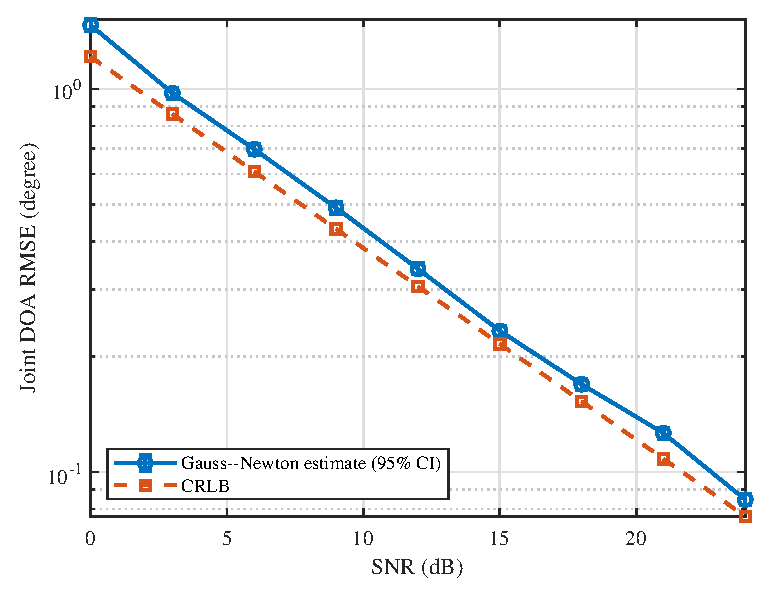
\includegraphics[width=0.95\linewidth]{simulation_results/ch5_spatial_reference_consistent_2026/results/fig_spatial_doa_rmse_crlb.eps}
    \caption{Joint DOA RMSE and the corresponding root CRLB versus SNR under the fixed spatial four-phase reference code. Error bars show 95\% confidence intervals.}
    \label{fig:doa_rmse_crlb_snr}
\end{figure}

Figure~\ref{fig:nmse_pilot_length} next examines the counting hierarchy in
\eqref{eq:pilot_length_requirement_hierarchy} for the per-element $L=2$
unstructured training problem. All operating points use prefixes of the same
QPSK pilot sequence and $10{,}000$ paired trials. The fixed-reference curve is
the scalar restriction of the spatial code to a representative receiving unit.
At $T_{\rm p}=2L$, its noiseless multistart success probability is about $0.54$;
at $T_{\rm p}=3L$, it exceeds $0.99$. The no-reference model retains its global phase ambiguity
and an approximately $3$~dB NMSE floor. Beyond the identifiability threshold,
additional measurements improve noise robustness, reaching about $-19.3$~dB
at $T_{\rm p}=48$. Success for an individual instance below $3L$ does not
establish global injectivity over the entire unstructured channel space.

\begin{figure}[t]
    \centering
    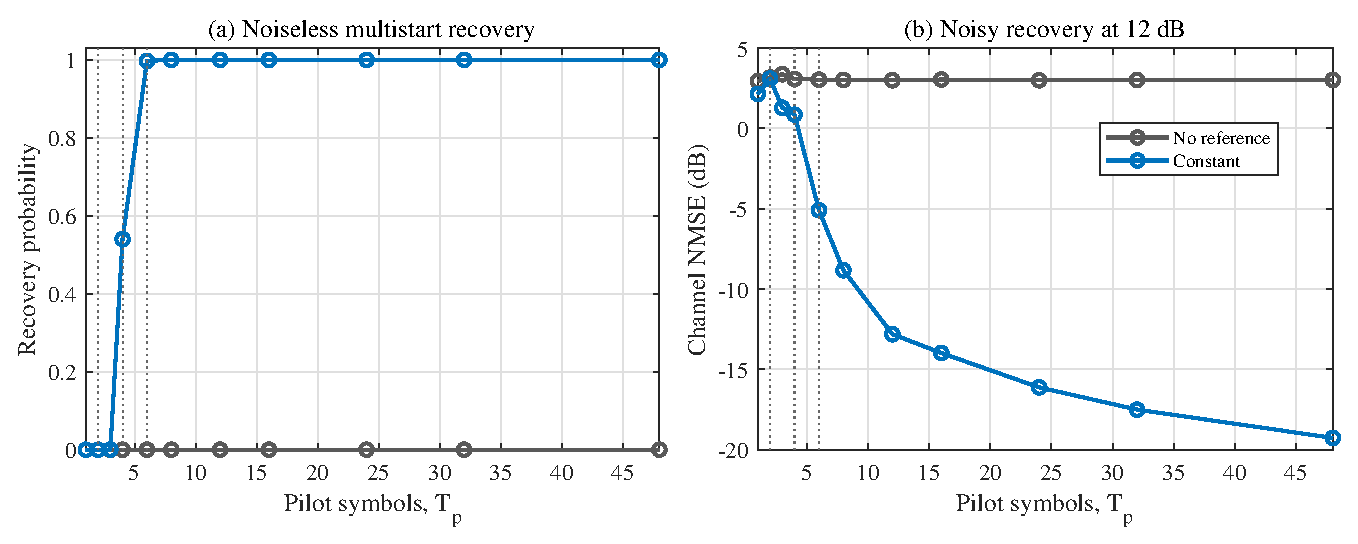
\includegraphics[width=\linewidth]{simulation_results/ch5_spatial_reference_consistent_2026/results/fig_spatial_pilot_identifiability.eps}
    \caption{Effect of pilot count for the two-user
    unstructured training problem: (a) empirical noiseless multistart recovery
    probability and (b) channel NMSE at $12$~dB, with and without a fixed nonzero reference. The vertical lines mark
    $T_{\rm p}=L$, $2L$, and $3L$.}
    \label{fig:nmse_pilot_length}
\end{figure}

Beyond the structural counting threshold, the training length required in
noise depends on the local estimation stability.  We therefore use the
Jacobian and CRLB analysis to decide whether additional pilots should be
acquired.  Figure~\ref{fig:stability_guided_training} compares this policy with
fixed short and long training, a noise-aware residual stopping rule, and an
oracle stopping rule based on the true channel error.  All policies use the
same nested QPSK pilot prefixes, the practical initialization in
Algorithm~\ref{alg:joint_gn_estimation},
and LM refinement; the coarse grid uses $0.5^\circ$ and $1^\circ$ spacings in
the polar and azimuth angles, respectively, and $\alpha_{\max}=2$ under the
adopted gain normalization. The experiment uses two users at polar angles
$19^{\circ}$ and $21^{\circ}$ with a common $5^{\circ}$ azimuth, the fixed
spatial phase map, candidate lengths $T_{\rm p}\in\{8,12,\ldots,40\}$, and
$300$ paired trials per SNR. The proposed policy selects the shortest prefix
whose predicted channel CRLB-NMSE is below $-25$~dB, DOA CRLB is below
$1^{\circ}$, and Jacobian normal-matrix condition number is below $5\times10^3$.

The residual rule stops near $T_{\rm p}=8$ even when the physical parameters
remain inaccurate: at $8$~dB it uses $8.33$ pilot symbols and yields
$-22.22$~dB NMSE. The proposed policy instead selects $30.92$ symbols and
reaches $-28.16$~dB. At $10$ and $12$~dB, it uses $20.04$ and $12.60$
symbols to attain $-28.13$ and $-28.34$~dB, respectively, and from
$14$~dB onward it selects essentially the shortest prefix. Fixed long training gives
the lowest NMSE but always uses $40$ symbols, whereas the proposed
overhead closely follows the oracle transition.  Thus, the stability analysis
detects information insufficiency that a small fitting residual alone does not
reveal and converts it into a direct accuracy--overhead gain.

\begin{figure}[t]
    \centering
    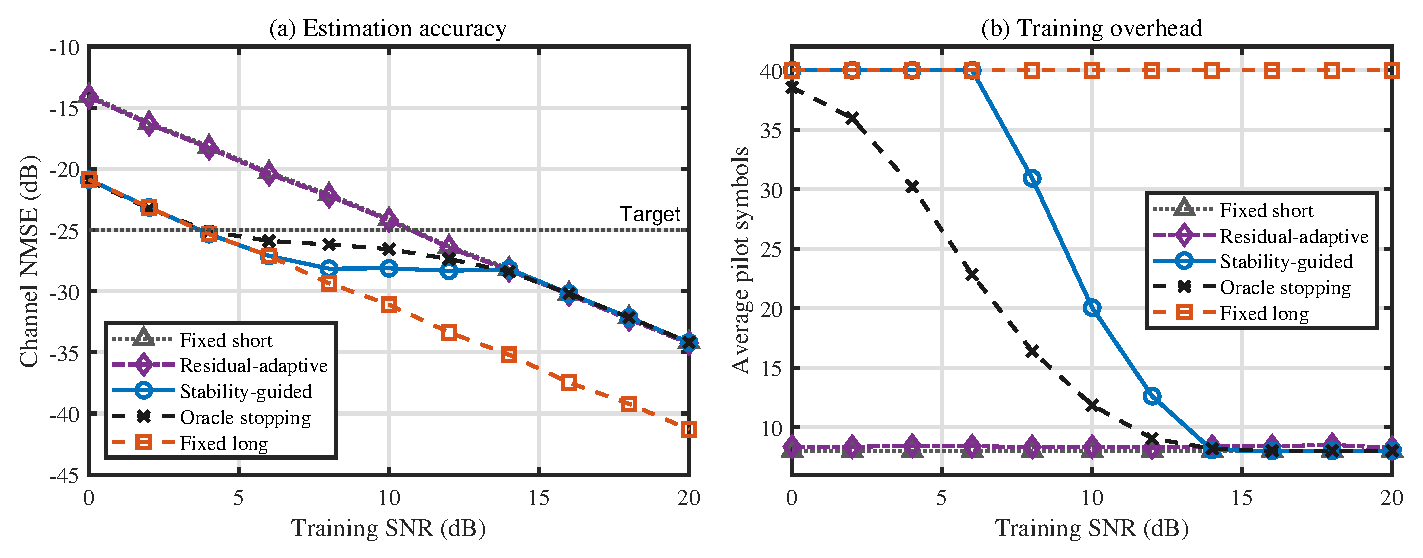
\includegraphics[width=\linewidth]{simulation_results/ch5_spatial_reference_consistent_2026/results/fig_spatial_stability_guided_training.eps}
    \caption{Stability-guided adaptive training with the practical
    Algorithm~\ref{alg:joint_gn_estimation} initialization: (a) channel NMSE
    and (b) average selected pilot
    symbols versus training SNR. The fixed-short and fixed-long schemes
    use $T_{\rm p}=8$ and $40$, respectively; oracle stopping uses the true
    channel error only as an unattainable benchmark. Each point averages
    $300$ paired trials.}
    \label{fig:stability_guided_training}
\end{figure}

\subsection{Symbol Detection Performance with Perfect CSI}

We isolate the detector from channel-estimation errors by constructing
$\mathbf G_{\rm d}$ from the true channel. Two QPSK users and the simultaneous
spatial four-phase map with $\rho=1.5$ are used. In
Fig.~\ref{fig:certified_gs_accuracy_complexity}(a), each point contains
$30{,}000$ symbol-vector trials. Exhaustive ML remains the accuracy benchmark,
while projected WF provides a gradient-based iterative baseline for the
linearized and GS detectors. At $-5$~dB, the ML, projected-WF, and certified-GS
SERs are $0.164$, $0.165$, and $0.214$, respectively. Weighting the pairwise
error probabilities in Theorem~\ref{thm:discrete_stability} by the normalized
Hamming distances and summing over all candidate pairs gives the analytical
SER union bound. It equals $0.333$ at $-5$~dB and approaches the ML curve in
the waterfall region.

Figure~\ref{fig:certified_gs_accuracy_complexity}(b) evaluates the stopping
test in~\eqref{eq:distance_certified_ml_test} using the same trials.
At low SNR the certificate is deliberately inactive and both iterative methods
approach the $25$-iteration budget. At $11$~dB, their average iteration counts
fall to $3.80$ for projected WF and $4.13$ for GS, and both are essentially zero
at $13$~dB once the initialized candidate lies inside the exact decoding
radius. A projected-WF iteration includes a gradient evaluation and
backtracking, whereas GS uses the precomputed closed-form back-projection.

\begin{figure}[t]
    \centering
    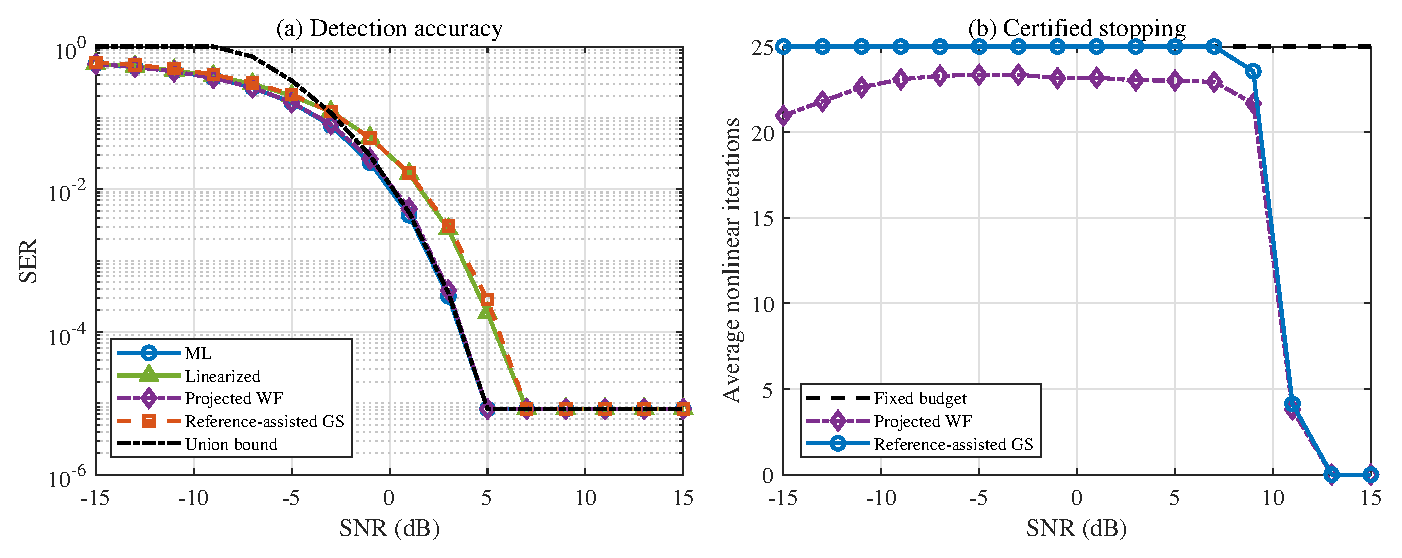
\includegraphics[width=\linewidth]{simulation_results/ch5_projected_wf_baseline_2026/results/fig_projected_wf_detection.eps}
    \caption{Perfect-CSI detection: (a) SER of ML, linearized, projected-WF,
    and reference-assisted GS detectors together with the analytical
    distance-spectrum union bound, and (b) their average nonlinear iterations
    under the exact $d_{\min}^{(E)}$ stopping certificate. Empirical SER points
    with no observed errors are omitted.}
    \label{fig:certified_gs_accuracy_complexity}
\end{figure}

To verify the pairwise theory directly, Fig.~\ref{fig:ser_vs_dmin} uses 32
equal-power fixed spatial phase maps spanning a broad range of normalized
minimum distances. For each map, Monte Carlo simulation is applied to its
closest candidate pair. The results follow the Gaussian expression in
\eqref{eq:pairwise_error_probability}, confirming that increasing the worst-case
intensity separation lowers the corresponding pairwise error probability and
validates $d_{\min}^{(E)}$ as a reference-design metric.

\begin{figure}[t]
    \centering
    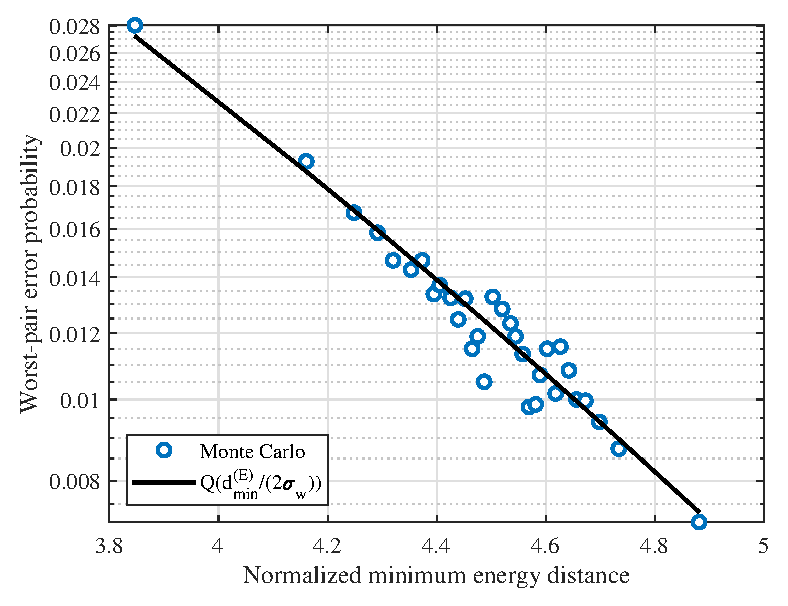
\includegraphics[width=0.96\linewidth]{simulation_results/ch5_spatial_reference_consistent_2026/results/fig_spatial_pairwise_error_vs_dmin.eps}
    \caption{Worst-pair error probability versus normalized energy-domain minimum distance over equal-power fixed spatial phase maps.}
    \label{fig:ser_vs_dmin}
\end{figure}

\subsection{End-to-End Symbol Detection with Estimated CSI}

We next propagate the channel estimates from the preceding adaptive-training
experiment to exhaustive data detection. The data SNR is fixed at $0$~dB, and
each of the $300$ independent training-noise realizations uses $200$ data
vectors. The observations are generated with the true channel, whereas each
estimated-CSI ML detector constructs its candidate templates from the
corresponding channel estimate. The
fixed-short, stability-guided, and fixed-long receivers differ only in the
pilot prefix used to form their CSI; the perfect-CSI curve identifies the data-noise floor.

At low training SNR, the stability rule requests the long prefix and closely
tracks fixed-long training. At $0$~dB, for example, it reduces the end-to-end
SER from about $0.18$ with eight pilots to about $0.14$, while the associated
channel NMSE improves from $-14.0$ to $-20.9$~dB. As training SNR increases,
the selected prefix shortens and all estimated-CSI curves approach the
perfect-CSI floor. This verifies that the stability test improves detection by
controlling channel-error propagation rather than by altering the detector.

\begin{figure}[t]
    \centering
    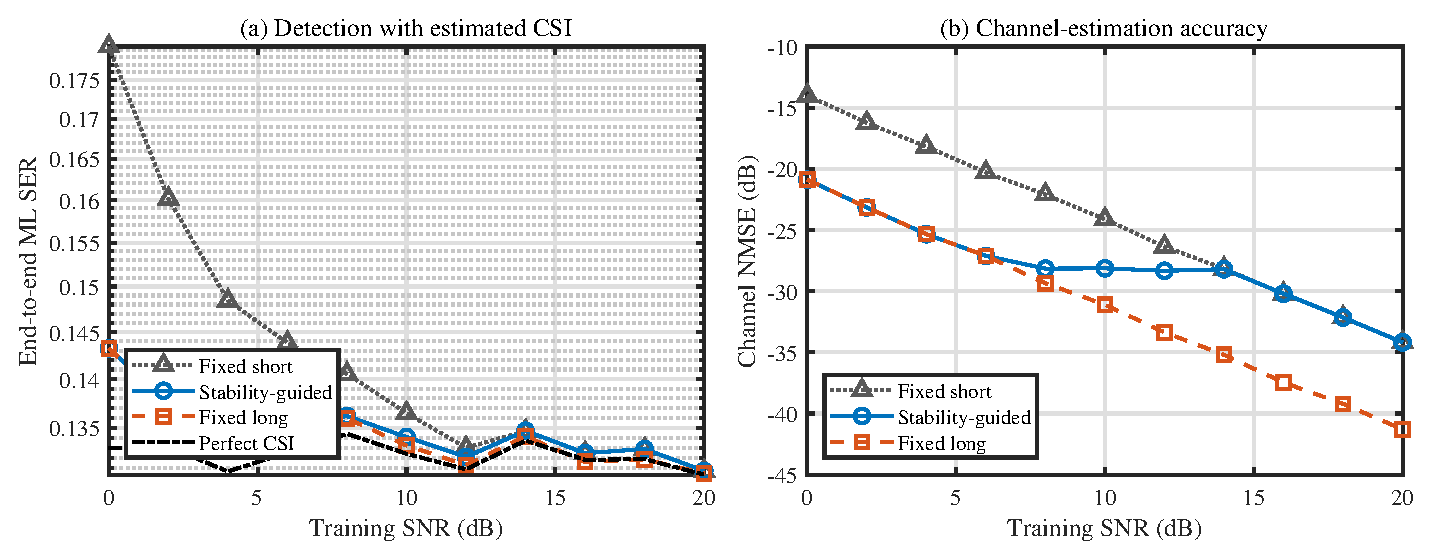
\includegraphics[width=\linewidth]{simulation_results/ch5_spatial_reference_consistent_2026/results/fig_spatial_end_to_end.eps}
    \caption{End-to-end comparison versus training SNR: (a) SER of the
    fixed-short, stability-guided, and fixed-long training policies with
    perfect-CSI ML as a benchmark and (b) their channel NMSE. The data SNR is
    $0$~dB.}
    \label{fig:theory_guided_end_to_end}
\end{figure}

\subsection{Effect of Surface Size and Angular Separation}

We next examine how receiving-surface size and angular separation change the
finite-alphabet decision margin. To compare configurations with different
numbers of observations, $d_{\min}^{(E)}$ is normalized by the root-mean-square
noiseless intensity. The two-user QPSK setting and fixed spatial four-phase map are
used unless otherwise stated.

At $-12$~dB, Fig.~\ref{fig:ris_element_measurement_diversity} shows that
increasing $N_{\rm r}$ from $4$ to $1024$ raises the normalized minimum
distance from $0.56$ to $19.61$ and lowers the ML SER from $0.693$ to $9.95\times10^{-3}$. This close
correspondence demonstrates the combined benefit of the enlarged aperture and
the increased number of intensity observations.

\begin{figure}[t]
    \centering
    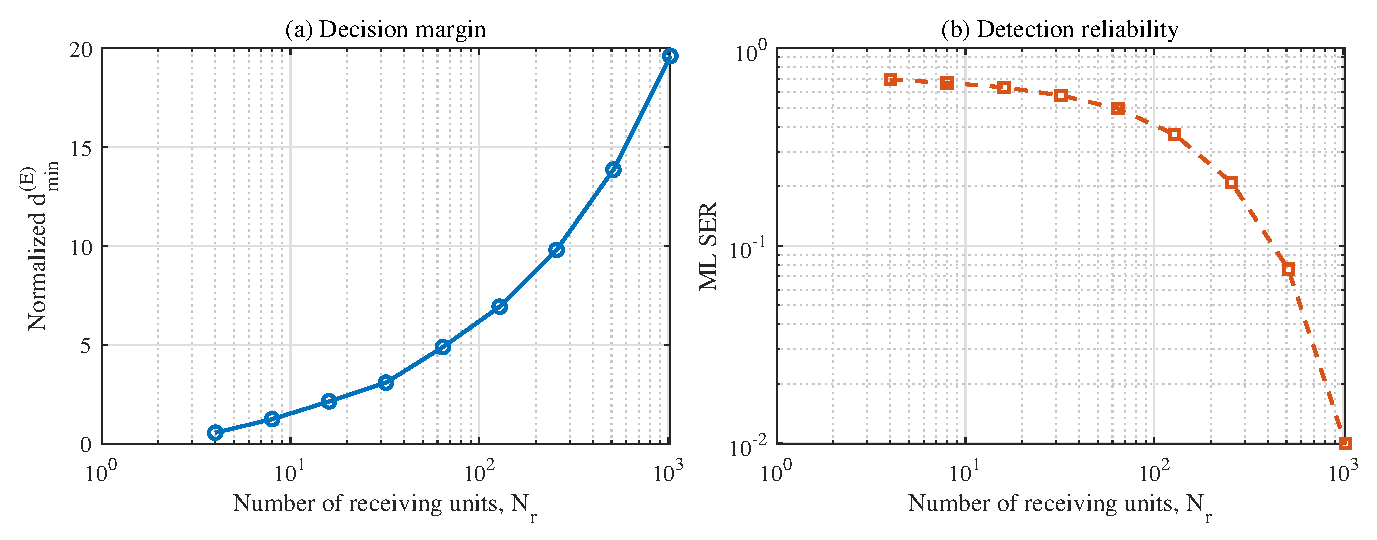
\includegraphics[width=\columnwidth]{simulation_results/ch5_spatial_reference_consistent_2026/results/fig_spatial_unit_diversity.eps}
    \caption{Combined effect of receiving-surface size and observation count on (a) the normalized energy-domain minimum distance and (b) perfect-CSI ML detection at $-12$~dB.}
    \label{fig:ris_element_measurement_diversity}
\end{figure}

Figure~\ref{fig:angular_separation_end_to_end} connects spatial conditioning to
detection. Increasing the separation from $0.25^\circ$ to $8^\circ$ raises the
normalized minimum singular value from $0.0209$ to $0.609$ and lowers the
perfect-CSI SER from $0.409$ to $0.248$ at $-6$~dB. The mild nonmonotonicity at
larger separations reflects finite-aperture sidelobes.

\begin{figure}[t]
    \centering
    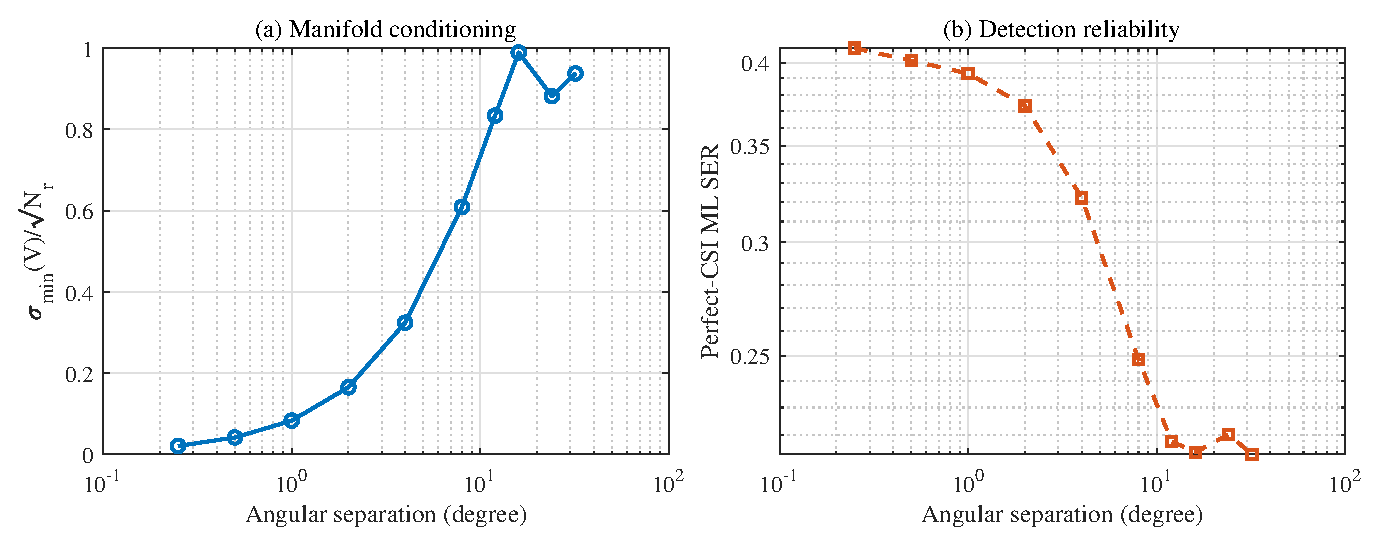
\includegraphics[width=\columnwidth]{simulation_results/ch5_spatial_reference_consistent_2026/results/fig_spatial_angular_separation.eps}
    \caption{Effect of user angular separation on (a) array-manifold conditioning and (b) perfect-CSI ML detection at $-6$~dB.}
    \label{fig:angular_separation_end_to_end}
\end{figure}

Together, these results show that surface size, observation count, and
array-manifold conditioning must preserve relevant field differences before the
reference-assisted projection can separate their intensities.

\subsection{Effect of the Reference-to-Signal Energy Ratio}

We finally examine the energy allocation in
Corollary~\ref{cor:balanced_energy_allocation}. The total average incident energy
per unit is fixed as $P_{\rm s}+P_{\rm b}=1$. Hence, sweeping the reference-to-signal energy
ratio ${\rm RSR}=10\log_{10}(P_{\rm b}/P_{\rm s})$ changes only the allocation
between the unknown and reference fields, rather than the detector power
budget. Figure~\ref{fig:reference_signal_energy_ratio} averages over $24$
phase-balanced fixed maps, each assigning every reference phase to $16$
receiving units, with $1500$ symbol trials per map and ratio. For each map, the
noise variance is calibrated at ${\rm RSR}=0$ and then held fixed throughout
the sweep.

Figure~\ref{fig:reference_signal_energy_ratio}(a) shows that the ensemble-mean
minimum distance is maximized near balance, at the sampled value
${\rm RSR}=-3$~dB for this constellation and channel. The shift from exactly
$0$~dB is consistent with \eqref{eq:pairwise_optimal_energy_split}, whose optimum
depends on the amplitude term $A_{ij}/B_{ij}$. The ML curves in panel (b) have
the corresponding bowl shape at all three noise levels. Thus, the relevant
design conclusion is not a universal $0$-dB optimum: severe imbalance in either
direction weakens phase-sensitive separation, while the preferred ratio can be
tuned from training data subject to detector dynamic range.

\begin{figure}[t]
    \centering
    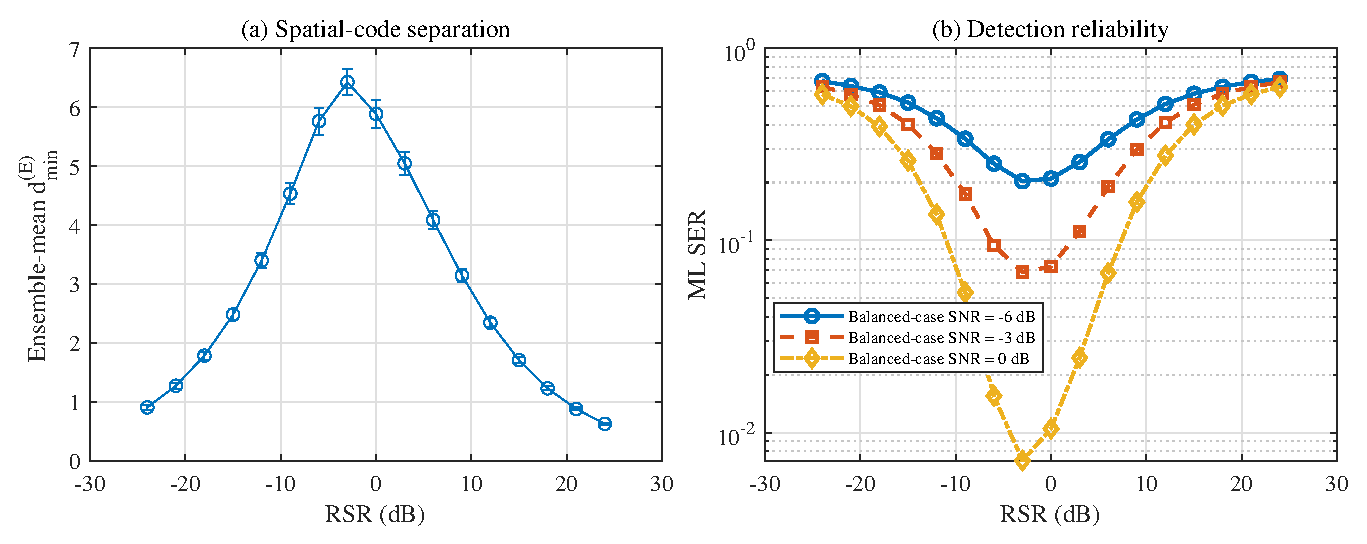
\includegraphics[width=\columnwidth]{simulation_results/ch5_spatial_reference_consistent_2026/results/fig_spatial_reference_energy_balance.eps}
    \caption{Effect of the reference-to-signal energy ratio under a fixed total incident-energy budget: (a) ensemble-mean minimum energy distance over phase-balanced spatial maps and (b) perfect-CSI ML SER at three balanced-case SNRs. Error bars show one standard deviation across phase maps.}
    \label{fig:reference_signal_energy_ratio}
\end{figure}


\FloatBarrier
\section{Conclusion}
\label{sec:conclusion}

This paper developed a reference-assisted RF holographic receiver for recovering complex channel and data information from intensity-only measurements. For the resulting affine intensity model, we established Jacobian-based uniqueness and stability conditions for continuous channel sensing and an energy-domain minimum-distance criterion for finite-alphabet detection. The analysis further revealed the roles of pilot diversity, spatial four-phase reference coding, and reference--signal energy balance. Guided by these results, we designed a two-stage receiver combining linearized initialization, stability-guided adaptive training, damped Gauss--Newton estimation, and distance-certified GS detection. Simulations under representative two-user far-field settings supported the predicted trends and showed that the adaptive scheme reduced the average pilot length from $40$ to $20.0$ at $10$~dB while attaining $-28.1$~dB channel NMSE. These results demonstrate the feasibility of recovering complex communication information without coherent I/Q acquisition.

% \section*{Acknowledgment}
% This work was supported in part by the National Science Foundation under Grant ECCS-2030250 and in part by the Semiconductor Research Corporation under Task 2810.075.

\bibliographystyle{IEEEtran}
\bibliography{references}     % 你的 .bib 文件名（不带扩展名）



\end{document}
